%\documentclass[letter]{article}
\documentclass[letter,12pt]{article}
\usepackage[letterpaper,right=1.25in,left=1.25in,top=1in,bottom=1in]{geometry}
\usepackage{setspace}

%\usepackage[utf8]{inputenc}   % allows direct input of accented and other special characters input directly (instead of \'a etc).
\usepackage[T1]{fontenc}      % what fonts to use when printing characters       (output encoding)
\usepackage{amsmath}          % facilitates writing math formulas and improves the typographical quality of their output
\usepackage{amssymb}          % extended symbol collection
\usepackage{url}              % adds line breaks to long urls
\usepackage[pdftex]{graphicx} % enhanced support for graphics
\usepackage[pdftex, hidelinks]{hyperref} % 

\usepackage[longnamesfirst, sort]{natbib}\bibpunct[]{(}{)}{,}{a}{}{;}

\usepackage{mathptmx}           % set font type to Times
\usepackage[scaled=.90]{helvet} % set font type to Times (Helvetica for some special characters)
\usepackage{courier}            % set font type to Times (Courier for other special characters)

%\usepackage{rotating}
%\usepackage{pdflscape}

\newcommand{\mc}{\multicolumn}

\usepackage{dcolumn}          % aligns tabular columns at decimal point---column type D{.}{.}{N decimal places}

\usepackage{arydshln}         % dashed lines in tables (usage: \hdashline, \cdashline{3-4}, 
                              %see http://tex.stackexchange.com/questions/20140/can-a-table-include-a-horizontal-dashed-line)
                              % must be loaded AFTER dcolumn, 
                              %see http://tex.stackexchange.com/questions/12672/which-tabular-packages-do-which-tasks-and-which-packages-

\graphicspath{{../graphs/}}   % double braces needed for this to work

%\usepackage{epigraph}         % write/format epigraphs


\begin{document}


\title{The effects of malapportionment, turnout, and gerrymandering in Mexico's mixed-member system\thanks{We are grateful to Jonathan Slapin, Chris Wells, to conference participants at the University of Houston (Nov.~14--15, 2014), and seminar attendees at the University of Florida (Mar.~13, 2015) for comments and critiques; to Drew Linzer and Javier M\'arquez for guidance to read their computer code; and to IFE's Cartography Department for sharing their experience with automated redistricting since 1996 and most of the data we analyze. We also acknowledge the support from the Asociaci\'on Mexicana de Cultura A.C.\ and CONACYT for this work.}}
\author{E.~Magar\footnote{Corresponding author: \url{emagar@itam.mx}} \\ \emph{ITAM} \and
        M.~Altman \\ \emph{MIT} \and
        M.P.~McDonald \\ \emph{UF} \and  
        A.~Trelles \\ \emph{Pitt}
      }
\date{\today}
\maketitle


% Author's info: Alejandro Trelles (lat44@pitt.edu) is a Ph.D. candidate in political science at the University of Pittsburgh, 4600 Wesley W. Posvar Hall, Pittsburgh, PA, 15260. Tel: +1(412)9790715. Micah Altman (escience@mit.edu) is Director of Research and Head/Scientist, Program on Information Science for the MIT Libraries, at the    Massachusetts Institute of Technology (MIT), E25-131, 77 Massachusetts Ave, Massachusetts Institute of Technology, Cambridge, Massachusetts, 02139. Tel: +1(585)4664224. Eric Magar (emagar@itam.mx) is associate professor of political science at ITAM, Río Hondo #1, Progreso Tizapán, México, D.F.,  01080. Tel: +52(55)6284000. Michael P. McDonald, Michael.mcdonald@ufl.edu, is associate professor of political science at the University of Florida, 234 Anderson Hall, Gainesville, Florida, 32611. Tel: +1(352)3920262.

\begin{abstract}
\noindent Reform since 1997 rid Mexico of the most flagrant distortions on representation. We study party bias and its sources in the plurality tier of the mixed system to elect one chamber of Congress. Our inquiry applies a procedure to measure three potential sources of party bias separately: substantial malapportionment, gerrymandering, and turnout. Monte Carlo simulations of recent elections offers empirical leverage for estimation. Results show that, relative to the right-of-center PAN, the formerly hegemonic PRI, but especially the left-of-center PRD, have enjoyed advantage in the votes to seats conversion. Analysis reveals how systematic and often substantive turnout-based bias in favor of the PRI has sometimes been countered by district boundaries substantively helping one or both other major parties. Despite nominally neutral district drawing, gerrymandering remains a key ingredient of the mix for party bias in representation.
\end{abstract}

% Search James Parker Smith and the Royal Commission on Systems of Election 1909 for cube law's origins
% Then an explanation of why we can't find it, despite substantial malapportionment: very large inter-election swings. 
% Slapin: Is is normatively bad to sacrifice 1 citizen 1 vote, or ok if that sacrifice done for other goals such as indigenous representation or municipal boundaries?
%
% Micah: use total votes instead of total population to measure malapportionment. Should capture which bastions exist, if they are packed, turnout differences (if measured against p18). 
% Mike: consejos distritales and staff are patronnage posts coveted by parties and bureaucrats, how does redistricting affect calculus. Blends well with the story of consejeros distritales as homeowners in cabecera that they wish not to change. 
% Other paper: touch issue of weights, units and components of cost function in general---rabbit burgers from how to lie with statistics, one unit of rabbit and one unit of cow... Eric: that humans beat the machine is proof that the algorithm stops at local minima quite easily. 

% Comment [Eric] Dropped this, may be useful for framing of for discussion
% \begin{tabular}{l|c|c|}
%                   & \mc{2}{c}{Would 2013 have reverted?}\\ \cline{2-3}
% State is          & yes                  & no \\ \hline
% over-represented  & df oax pue sin       & bcs col\\ \hline
% under-represented &  cps gua que qui tam & ags bc cam coa dgo\\ \hline
%                   &                      & cua gue hgo mic mor  \\ 
% on target         & jal mex ver          & nay nl san son tab  \\ 
%                   &                      & tla yuc zac \\ \hline
% \end{tabular}

\onehalfspacing

\noindent Party bias is an asymmetry in the translation of votes to seats. The large-party premium typical of the plurality rule---the other classic quantity of interest to assess electoral systems\footnote{See, for example, \citet{rae.1967,tufte1973seatsVotes,erikson1972malapportionment,dahl.1956prefDemoc,gudgin.taylor.1979seatsVotes,taagepera.shugart.1989,taagepera.CubeLaw.1973,king.1990elRespBiasMultiparty,king.browning1987biasRespUS,gelman.king.1994EvalElSysRedis,calvo.roddenMultipartyPlurality2015,calvo.micozzi.govReform.2005}.}---is, in constrast, symmetric: \emph{any} top vote earner receives more seats than it is worth in votes. In this article we trace the forces that make party bias distort the system of representation by rendering seats cheaper for some parties than for others. 

Introduce the distributional, the turnout, and the malapportionment components of party bias. 

Mexico is a good laboratory to search for these forces...

%\noindent A classic approach to assessing electoral systems is the derivation of vote--seat curves. These curves capture how votes in general elections are converted into parliamentary seats, and thus are designed to evaluate the most fundamental function of electoral systems \citep{lijphartElSysPtySys.1994}. Particular attention has been given to plurality systems and the ways in which the vote--seat curve departs from proportional representation. 

Mexico's lower chamber of Congress has been elected with a mixed-member electoral system for decades. Systems of this nature give voters a direct role in the election of representatives from single-member districts (SMDs), while also using some form of proportional representation (PR) to improve the odds that parties will receive about as many seats as they are worth in votes \citep{shugart.wattenbergIntro2001}. Underneath the PR-tier lies a standard plurality system. As in all plurality systems, we suspect strong distortions in the form of party bias to be arising in the SMD-tier. Substantial malapportionment, which has never disappeared in Mexico, is one cause for concern. But other factors---namely gerrymandering and district turnout differentials---may in fact contribute to bias the system further in favor of one party or another.   

Studying this requires a method to measure party bias and to assess how much of it is due to different sources. A model by \citet{king.1990elRespBiasMultiparty} generalizing the fit of a vote--seat curve including party bias provided the estimators. A procedure by \citet{grofman.etalBiasMalapp.1997} shows how to decompose estimates of party bias into three additive components. Using this general method (devised for a two-party system) in combination with King's model surmounted the obstacle of multiparty competition in Mexico. A final obstacle for estimation was the small number of elections celebrated since the system became democratic. Following recent work by \citet{linzerSeatVoteElasticity2012}, we overcame this by means of Monte Carlo draws, producing a large number of simulated national election outcomes consistent with the observed district-level distribution of partisan support. 

The paper is organized thus. Section 1 discusses partisan bias, three sources behind it (the distributive-, the turnout-, and the malapportionment-based), and how operationalizing parties' national vote shares in slightly different ways clear the way to measure them empirically. Section 2 investigates malapportionment in Mexican elections, showing that it is substantially due to belated redistricting---when carried five or more years after the census, as has been done, population information is outdated. Section 3 derives expectations of bias from the partisan model of electoral regulation. District boundaries in Mexico are not drawn by politicians but by experts under the aegis of a collegiate electoral regulator where all three major parties share power \citep{estevez.magar.rosas.2008}. This removes suspicions of the flagrant manipulation such as partisan gerrymandering. Section 4 describes estimation methods and section 5 elaborates on our data. Section 6 reports our party bias results, both in terms of raw party bias and in terms of its three, additive components. Section 7 concludes. 

% \section{How to read a map}

% A new map is a full description of district boundary changes. The common way to visualize maps is on paper. We look at them differently, with focus not in the physical lines and their relation to landmarks and geographic accidents, but in their political consequences. Putting the 2006 map and the 2015 final proposal drawings side to side reveals boundary shifts. But unless the drawing is quite data rich, or your command of political geography is outstanding, assessing even superficial effects of boundary changes visually is a challenge. 

% \begin{table}
% \begin{center}
%   \begin{tabular}{lrrrrr}
%   Similarity between                   &   min  &  25\%  & median &  75\% &  max \\ \hline
%   initial 2015 proposal and status quo & 0.128  & 0.419  & 0.584  & 0.755 &  1   \\
%   final 2015 proposal and status quo   & 0.125  & 0.437  & 0.643  & 0.805 &  1   \\
%   final and initial 2015 proposals     & 0.174  & 0.705  & 0.967  & 1     &  1   \\
%   \end{tabular}
%   \caption{District similarity of the 2015 map}\label{T:simIndex}
% \end{center}
% \end{table}

% A similarity index \citep[][:15--7]{cox.katz.2002} illustrates our method, offering ground for systematic assessment of a pair of maps. Measurement identifies the parent district or single largest contributor of population to every new district. The $s$imilarity index divides the population that $p$arent and $n$ew district share in $c$ommon by their joint population: $s = c / (p + n - c)$. The range is zero (district shares no population at all with parent) to one (districts are identical). The statistic conveys an intuitive measure of how much districts changed in the new map. Table \ref{T:simIndex} describes 2015 map changes against the status quo (the 2006 map), including the technical committee's initial proposal for party assessment and the revised, final proposal sent for approval. Also compared are the final and initial proposals themselves. % Slapin wrote: how is population measured?

% Six percent of districts entertained no change in boundaries whatsoever vis-\`a-vis the status quo (18 districts in the initial proposal, 19 in the final),\footnote{Slapin wrote: how did their populations change?} and twice as many had at least nine-tenths of the population in common (40 districts in the initial, 44 in the final proposal). Inspecting which districts were \emph{a priori} chosen for marginal or no change might reveal systematic distortions of the automated redistricting algorithm. Party feedback left 39 percent of districts in IFE's first proposal intact, and 62 percent with up from nine-tenths of the population in common. Inspecting which districts the parties targeted for major amendment --- presumably a partial reinstatement of a preferred status quo district --- should shed further light into the subject. Note how median district similarity with the 2006 map augmented from first to final proposal. So did the third quartile. Accepted counter-proposals therefore reconstituted portions of status quo districts. This seems consistent with a view where parties protect strongholds that the algorithm may have split, but further analysis must be done---these are exciting lines that future versions of this project should pursue!

%%%%%%%%%

% Mexico had its first population census in 1900. It has done them every decade since 1920, and every five years since 1990. Such short inter-censal periods offer relatively precise estimates of how many live in boroughs in every corner of a country with still rapidly changing demographics. This official and public data is priceless for planners of all stripes, marketers, and researchers, to name a few. 

% But not everyone has taken advantage of the data. Redistricters in the last decades are among them, routinely shunning fresh population data availability. Part of their reluctance finds explanation in a Constitution mandating the use of decennial censuses, not lustrum population counts, to do their job; with no attempt to estimate population change since the census is published; and, unlike the U.S., no obligation to redistrict as soon as a new census is available. But much of the blame falls on legislators, parties, and electoral regulators who have, to larger or smaller extent, but systematically lagged behind the constitutional obligation to ensure equal representation when updated information has become available. 

% To get an idea of this, consider that information used to draw a new map for the 1979 congressional was nearly a full decade old upon the map's inauguration. Rural flight was probably at its peak then. That same map had missed nearly 25 years of demographic change when it was last used to translate votes into seats, in 1994. But the problem has carried over to the democratic era. The first map after transition was drawn with seven year old data. Had the lustrum count been used instead of the general census, the lag would have dropped to two years. And for reasons discussed below, when the 2015 midterm congressional election takes place, a decade-and-a-half gap will separate the map and actual district populations. 

% Malapportionment---when sparsely populated areas get the same representation as the more densely populated ones---arises as a consequence. This raises normative questions on the value of a vote in representative democracy \citep{cox.1987,balinskiYoung2001FairRep,dahl.1972}. But positive questions are no less important, as malapportionment may bias representative government in important ways. If some party or parties tend to be stronger in the smaller districts, they will enjoy undue influence in policy. With the PRI's still solid bases of support in Mexico's countryside \citep{amesMex.1970,magar.1994}, the question of party bias arsing from malapportionment merits closer scrutiny. 

% This paper starts with a description of the redistricting process in use since 1997. Automated redistricting in consultation with parties rid Mexican districts of the most flagrant distortions on representation, but problems remian. Next, the paper inspects one such problem: legislative malapportionment. The problem is shown to be substantive and systematic: by our estimates, in 2015 the most populated district will be four times larger than the least populated. The developments that have led to this situation are discussed. We next turn to some of its consequences for representation, with analysis of two distortions of scholarly interest: party bias and responsiveness (or large party bias). Surprisingly, our estimates reveal no systematic party bias, but responsiveness is huge. [In future incarnations, the paper will also relate the party bias and responsiveness estimates to measures of malapporionment, in search of an association at the state level. A discussion of how inter-election volatility may trump the effects of malapportionment will also be in order.]

% Taking district map drawing out of the hands of politicians does not, as \citet{johnstonRedistrictingInBritain2003} notes, necessarily ensure a fair result, however. 

\section{Sources of party bias}

% plots prepared in analizaEscenarios.r
% [Micah]: we should have replication data files available in Dataverse, and cite these... 
\begin{figure}
\begin{center}
\begin{tabular}{cc}
    % (a) & (b) \\
    % 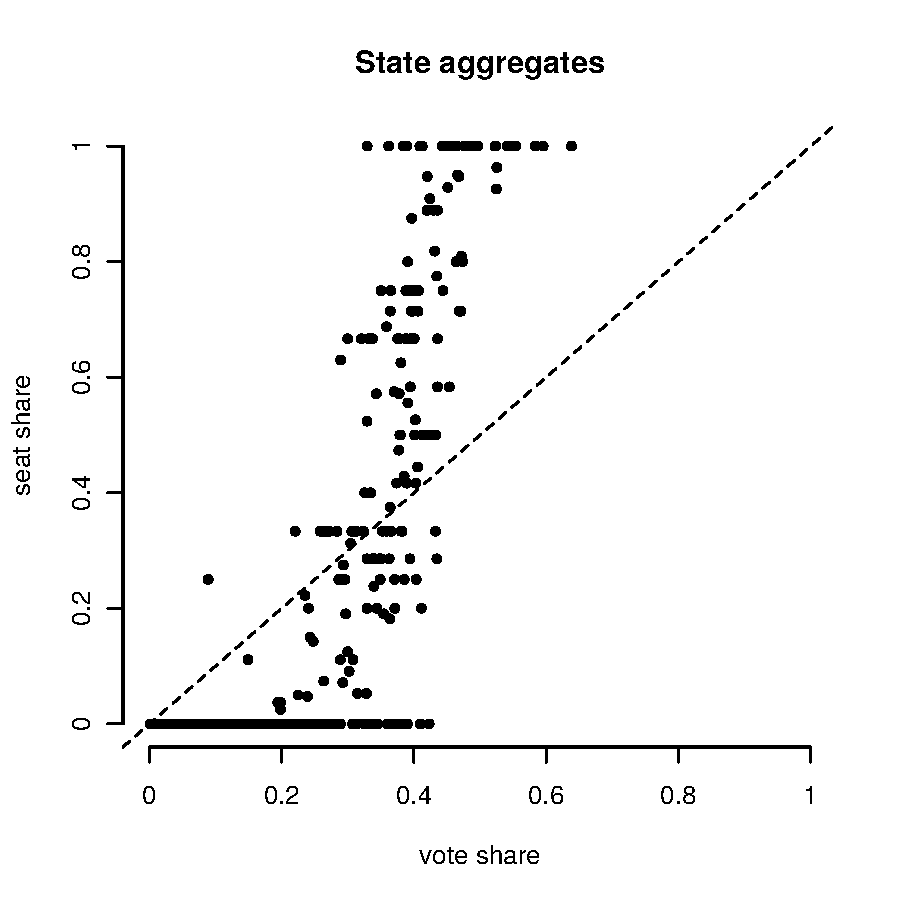
\includegraphics[width=.48\columnwidth]{resXedo20062012sh.pdf} &
    % 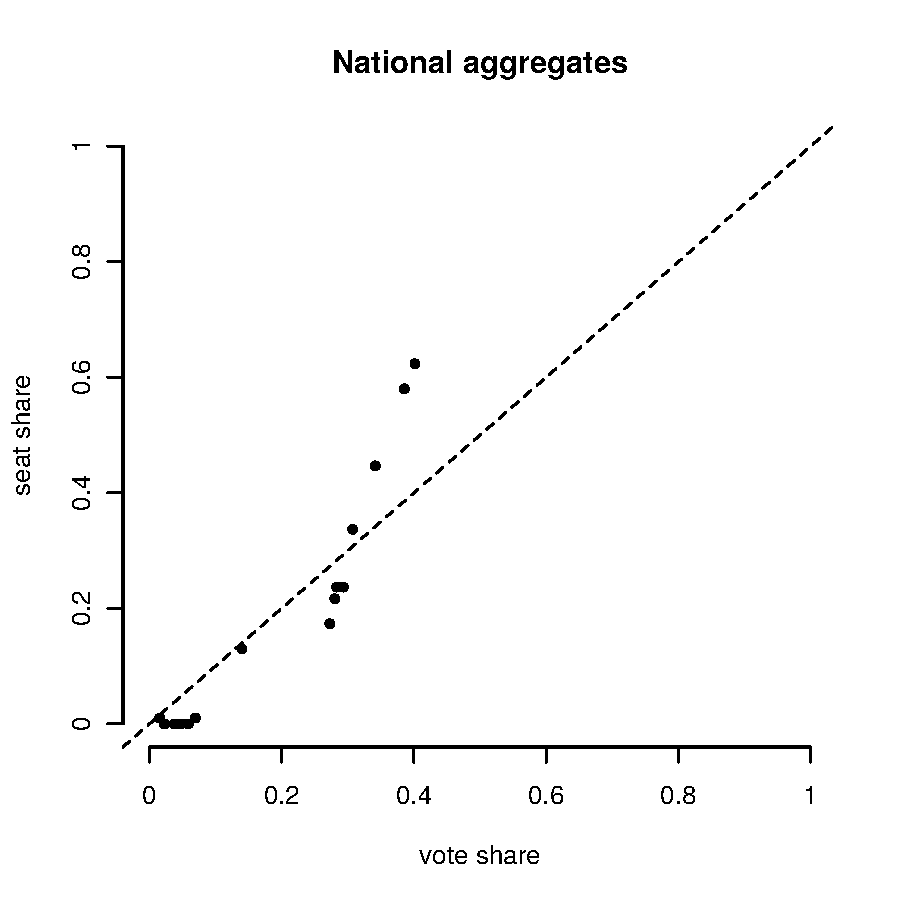
\includegraphics[width=.48\columnwidth]{resNal20062012sh.pdf} 
    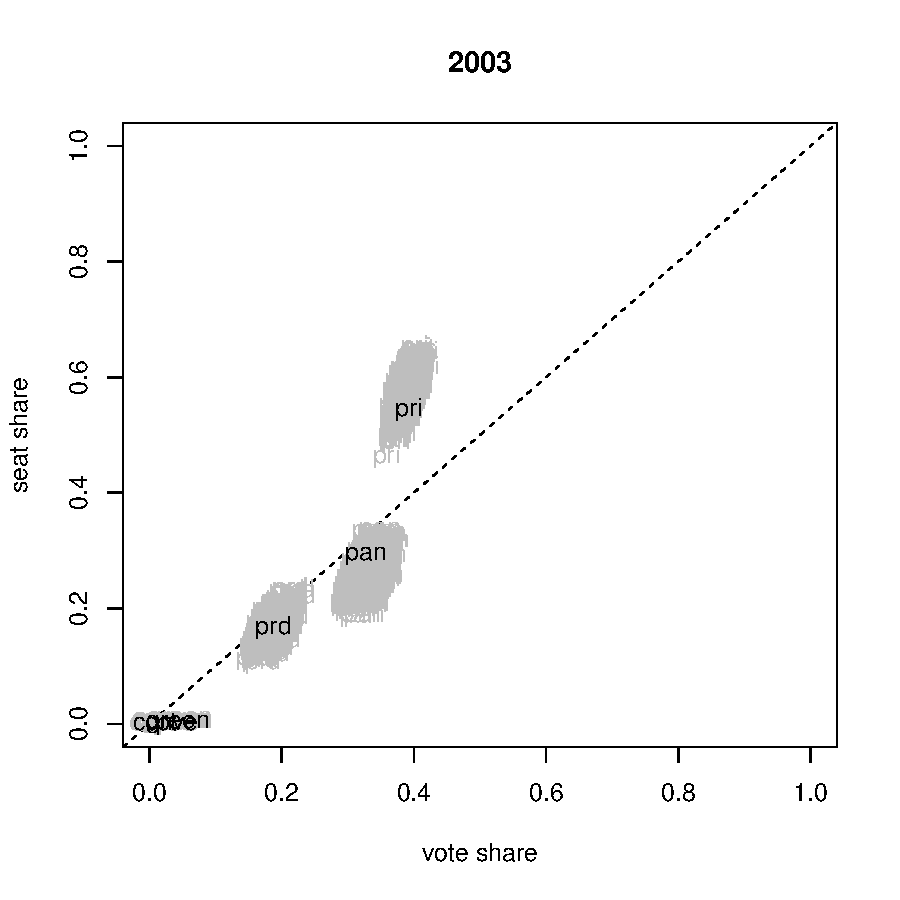
\includegraphics[width=.48\columnwidth]{vs2003.pdf} &
    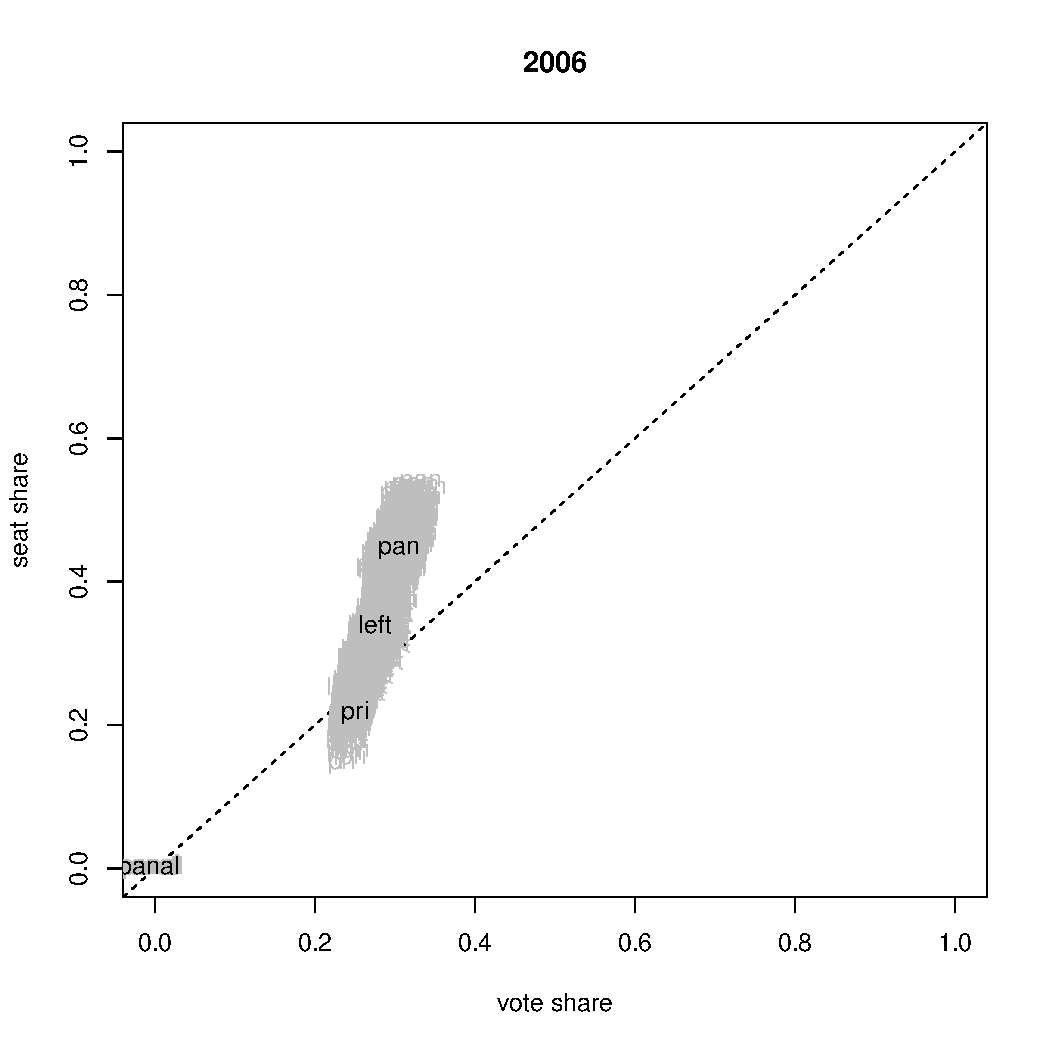
\includegraphics[width=.48\columnwidth]{vs2006.pdf} \\
    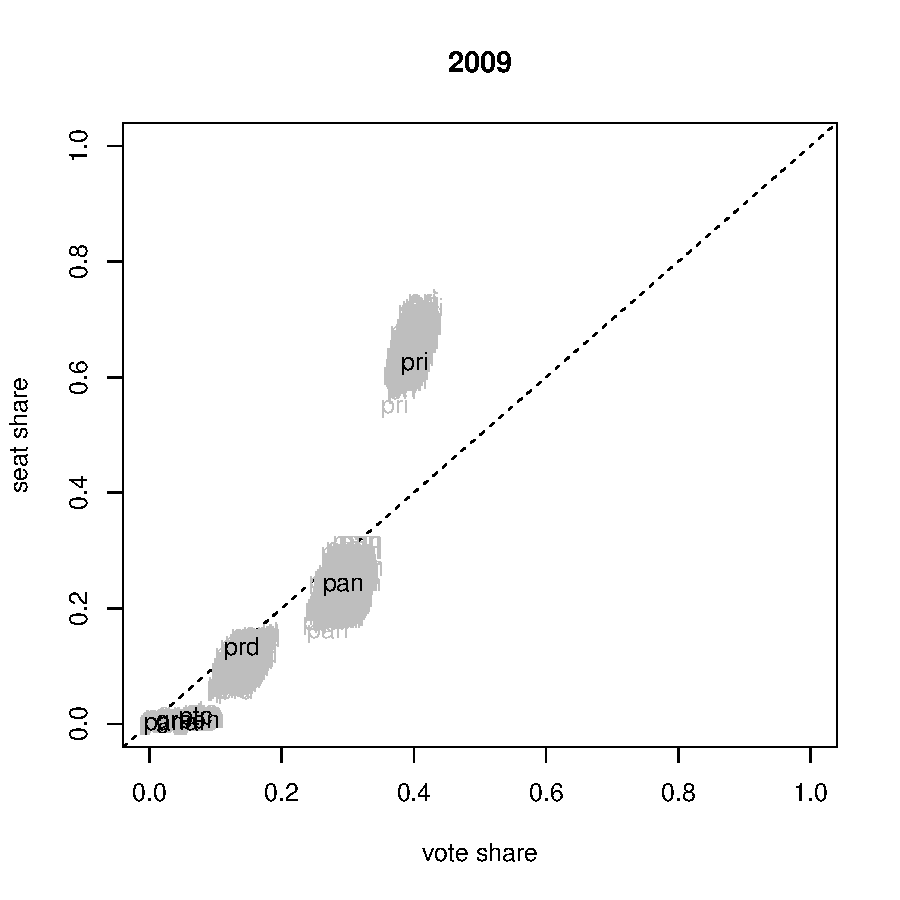
\includegraphics[width=.48\columnwidth]{vs2009.pdf} &
    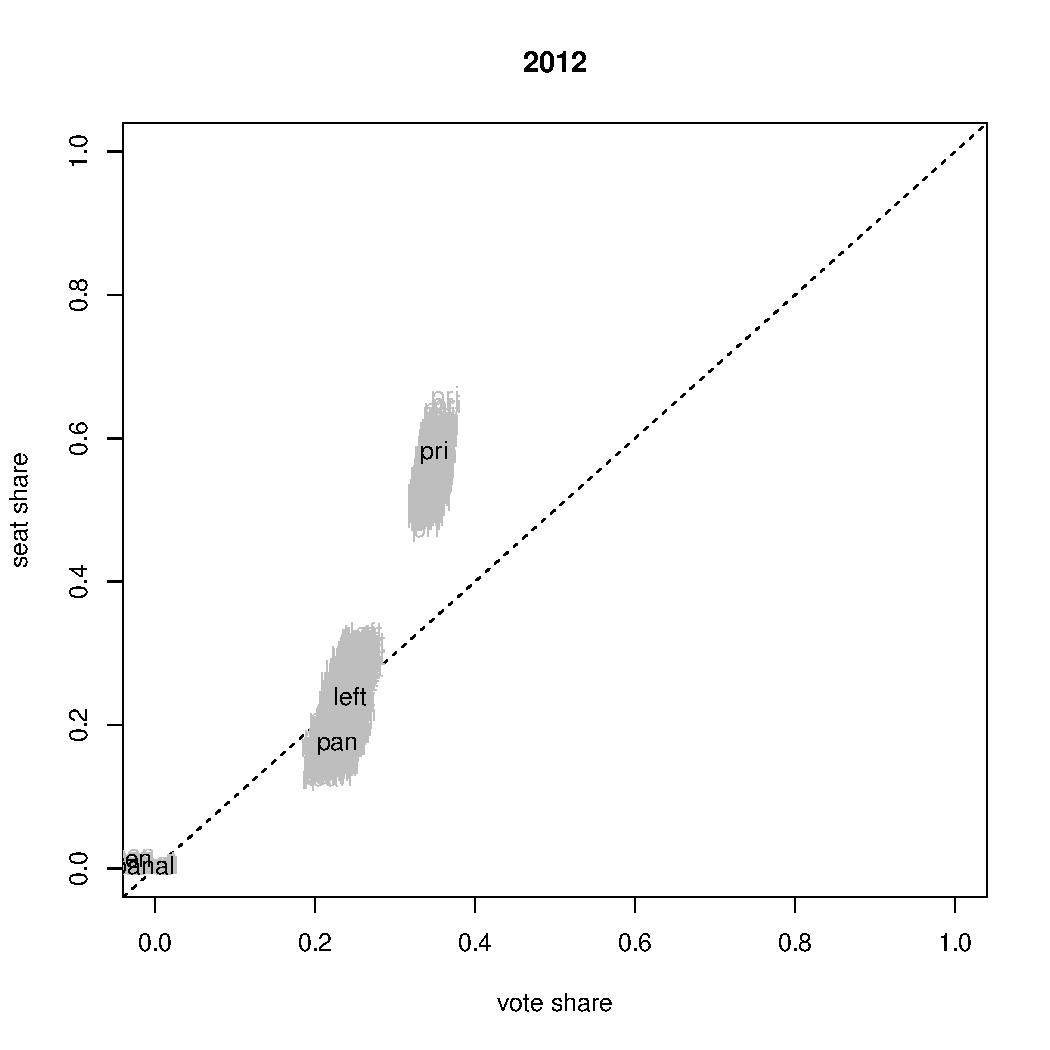
\includegraphics[width=.48\columnwidth]{vs2012.pdf} \\
\end{tabular}
\caption{Votes and plurality seats in the 2006, 2009, and 2012 federal deputy elections. Panel (a) reports state aggregates and each point is a party-state-year. Panel (b) reports standard national aggregates and each point is a party-year. Source: prepared with data from \url{www.ine.org.mx}.}\label{F:seatsVotes}
\end{center}
\end{figure}

Consider the relation between congressional party votes (x-axis) and seats (y-axis) portrayed in Figure \ref{F:seatsVotes}. Panel (a) relates shares at the state level (i.e., votes/seats won by the party in each of the state's federal districts, summed and divided by the total votes/seats in the state) and panel (b) at the national level (i.e., 300-district aggregates). Each point reports one party's vote-seat relation at the unit of aggregation in one election between 2006 and 2012. For instance, the dot floating to the left of the cloud and above the dashed diagonal line in panel (a) is the Green party in the state of Chiapas in 2012, where it won 3 out of 12 seats. The chart shows that 9 percent of the vote statewide awarded the party 25 percent of the seats, an outstanding achievement for any party. Both clouds manifest a steep upwards slope characteristic of plurality systems \citep{taagepera.CubeLaw.1973}.\footnote{Adding the excluded PR seats would level the slope considerably. Doing this would be easy with national aggregates. It is not evident how to carry it with state aggregates, since PR seats are awarded in five second-tier districts grouping several states each.} Points below the diagonal indicate under-representation, those above over-representation. Differences are notable among major parties: the PRI achieved over-representation in three-fifths of election-states in the period, the PAN in two-fifths, and the PRD in one-fourth only. Might the system confer undue advantage to the PRI? %Colors distinguish the parties: PAN is blue, PRI is red, PRD is gold, Green is green, among others. 

\subsection{Two classes of distortion}

% [Micah]: This section seems to be a digression. Would it be possible to put this in an appendix, and transition directly to next subsection.
% [Eric]: Agree, next version should shorten.

Undue advantage is known, in the specialized literature, as partisan bias, and is one goal that strategic redistricters pursue. It is not, however, alone: scholarship highlights district responsiveness, also known as majority premium, as another goal. These ought to be distinguished \citep[this explication draws heavily on][, ch.\ 3]{cox.katz.2002}. Partisan bias helps the beneficiary buy seats with fewer votes than others. Because seat distribution is a constant sum game, bias in favor of someone always implies bias against someone else. One way of introducing party bias in district lines is with the conventional redistricting strategy known as packing: group your adversary's voters in few districts, wasting votes to win unnecessarily safe seats, thus raising the price of victory. Responsiveness, on the other hand, is the feature granting a seat bonus to large parties. Maximal responsiveness occurs within each SMD in isolation: the winner takes all, the rest nothing. The same could be achieved in a whole state by drawing lines so that every district is representative of the state's electorate (Cox and Katz's microcosm strategy). The party with most votes statewide wins every seat, maximizing the vote responsiveness of the proposal. 

Formalizing party bias and responsiveness reveals how these district characteristics relate and opens the way towards their estimation. The two-party case is simpler \citep{taagepera.CubeLaw.1973,tufte1973seatsVotes,king.browning1987biasRespUS} and extends to multiparty competition. It is a generalization of the cube law stipulating that 

\begin{equation}\label{E:kingBi}
 \frac{s}{1-s} = e^\lambda *  \left(\frac{v}{1-v}\right)^\rho \iff
 \texttt{logit}(s) = \lambda + \rho *  \texttt{logit}(v)
\end{equation}\label{E:cubeLaw}

\noindent where $s$ is the seat share that the left party won with vote share $v$; $\lambda$ is the left party's bias relative to the right party (positive values favor the left, negative values favor the right); and $\rho$ is the districts' responsiveness. With $\lambda=0$ a system with no party bias ensues. Figure \ref{F:lambdaRhoEx} shows how the parameters affect the vote-to-seats conversion. 

% comment [Mike] how do multiple parties affect bias/responsiveness estimates, compared to two-party setting? I would expect that a party would often need less than 50% of the vote to win 50% of seats due to many parties receiving votes in single-member districts.

\begin{figure}
\begin{center}
    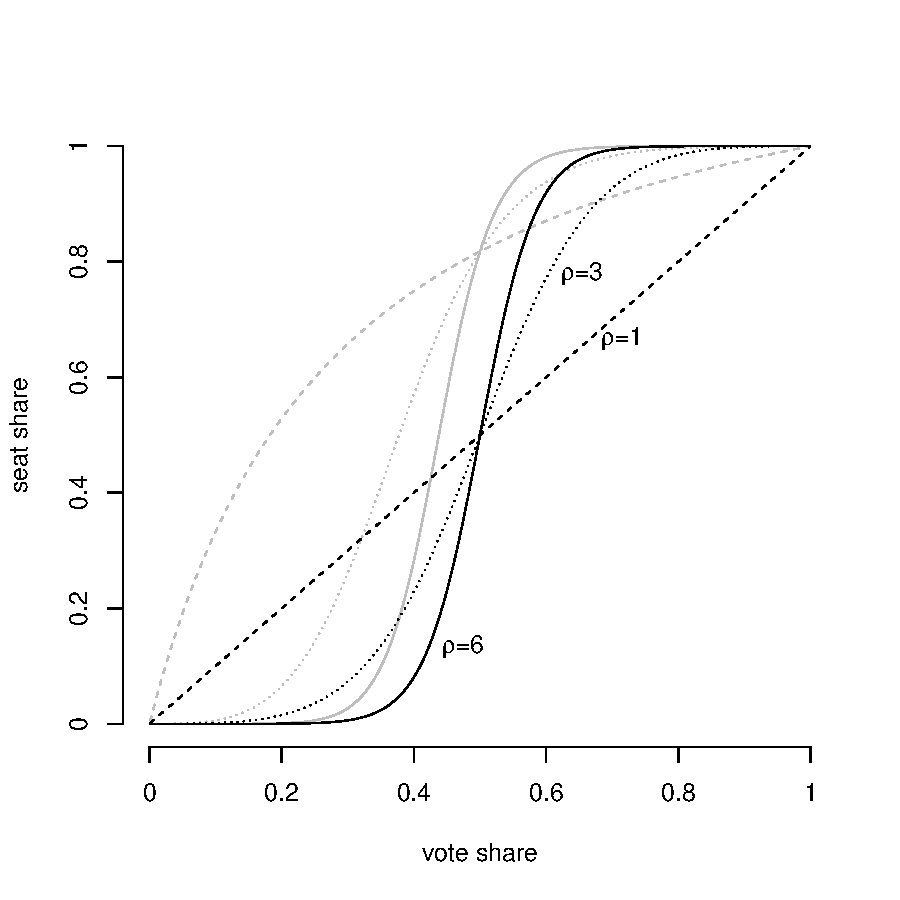
\includegraphics[width=.55\columnwidth]{rhoExample.pdf} 
\caption{Illustration of model parameters. Party bias is set to $\lambda=0$ in non-grey lines. Grey lines replicate the colored ones with $\lambda=+1.5$.}\label{F:lambdaRhoEx}
\end{center}
\end{figure}

Non-gray lines lack party bias to illustrate variable responsiveness. A system with $\rho=1$ is perfect PR, the ideal type against which real districts are often contrasted. It appears as the dotted green diagonal: every party winning $x$\% of the vote gets, precisely, $x$\% of seats. $\rho=3$ characterizes the classic cube law, the red curve over-representing the winner (points above the diagonal). Here a party with 55\% of the vote earns two-thirds of the seats, but with 33\% it earns only one-tenth of the seats. As responsivity heightens, the curve grows steeper, until barely crossing the majority threshold suffices to win all the seats available. 

\subsection{Separating sources}

Party bias is asymmetric treatment of parties in the vote--seat conversion. Grey lines replicate the values of $\rho$ just discussed but with $\lambda = +1.5$ added. Bias in favor of the left party achieves a leftward pull of lines. In other words, a bias-favored party will require less effort to reach the threshold for large-party over-representation, cooking artificial parliamentary majorities with substantially less than a vote majority---as routinely occurred in the United Kingdom since the 1970s. (The grey dotted line demonstrates how, due to logit links in Equation 1, party bias also reshapes the function's trace.) %When present, parties winning identical vote shares nationwide earn different seat shares. 

At the root of party bias in systems with multiple districts are differences in the geographic concentration of parties' vote strength. One party with 20 percent of the vote nationwide evenly spread across districts may fail to win a single seat, yet another with much less support but concentrated in few districts will, in fact, get seats. At the same time, vote concentration by larger parties leads to vote (and seat) wasting \citep{calvo.roddenMultipartyPlurality2015}. In the end, several forces add up and interact to yield party bias \citep{gudgin.taylor.1980decomposeBias}. Analysis of the components of party bias 

\citet{grofman.etalBiasMalapp.1997} demonstrate that what we shall now call \emph{raw party bias} ($\lambda$) has three clear and distinct sources and offer a procedure to separate empirically the independent contribution of each. Our analysis applies the GKB method to recent Mexican elections.\footnote{Other elements highlighted by \citet{gudgin.taylor.1980decomposeBias} that our analysis of raw party bias ignores are the cube-law's bonus, large third-party votes, and possible interactions between all the elements. The bonus is, in fact, captured by the system's responsiveness parameter and therefore distinct from party bias in our framework (more on this below). \citet{calvo.2009roadToPR} models departures from bipartism explicitly. Interactions remain interesting venues for future research.} The first source of party bias is \emph{distributional} (or vote wasting). It corresponds to partisan support differently spread across districts mentioned above. Vote wasting may be caused intentionally through gerrymandering (e.g., packing your opponent's support in few districts), but it may also arise by the accidents of geography (e.g., when districts do not cross state boundaries and the state is a party stronghold). The second source of party bias is differential \emph{turnout} across districts. Those who abstain from voting are passively lowering the bar to win a district's seat. Parties stronger in the lower turnout districts will achieve victories with fewer votes than adversaries, improving their votes:seats ratio. Turnout differentials arise when correlates of participation, such as socio-economic status, vary systematically across districts, or when parties mobilize more effectively in some areas than others \citep{rosenstone.hansen.1993}. The third source of party bias is \emph{malapportionment}. 


% [ERIC] Follows Micah's suggestion to have vote total add to same in each scenario. This makes each scenario's difference stand out, but raw vote numbers are larger and less round than they were... 
\begin{table}
\centering
% %\newcolumntype{d}[1]{D{.}{.}{#1}} % D column with 1 decimal spaces default, usage d{2} for two spaces
\newcolumntype{d}{D{.}{.}{2}} % D column with space for 2 decimal spaces
\begin{tabular}{lrdrrrrddrrrrdd}
          &              &                  &  \mc{3}{c}{Raw votes}      &&  \mc{2}{c}{Vote shares}        && \mc{2}{c}{Seat shares}\\ \cline{4-6} \cline{8-9} \cline{11-12}
%         &  (d)         &    (c/d)         &  a        &  (b)  &  (c)   && \mc{1}{r}{a/c}&   b/c          \\
Districts &  Pop.        &\mc{1}{r}{Turnout}&  left     & right&  total  &&\mc{1}{r}{left}&\mc{1}{r}{right}&&\mc{1}{r}{left}&\mc{1}{r}{right}\\ \hline
\mc{9}{l}{~~\textbf{Distributional-based party bias only}}                                                 && &     \\    
1 and 2   &  420         &   .5             &  147      &  63  &  210    &&   .\textbf{7} &   .\textbf{3}  && 1 & 0 \\
3, 4 and 5&  420         &   .5             &  84       &  126 &  210    &&   .\textbf{4} &   .\textbf{6}  && 0 & 1 \\ \hdashline
nationwide&  2100        &   .5             &  546      &  504 &  1050   &&   .52         &   .48          &&.4 &.6 \\ \hline
\mc{9}{l}{~~\textbf{Turnout-based party bias only}}                                                        && &     \\
1 and 2   &  420         &   .\textbf{70}   &  200      &  100 &  300    &&   .67         &   .33          && 1 & 0 \\
3, 4 and 5&  420         &   .\textbf{35}   &  50       &  100 &  150    &&   .33         &   .67          && 0 & 1 \\ \hdashline
nationwide&  2100        &   .5             &  550      &  500 &  1050   &&   .52         &   .48          &&.4 &.6 \\ \hline
\mc{9}{l}{~~\textbf{Malapportionment-based party bias only}}                                               && &     \\ 
1 and 2   & \textbf{600} &   .5             &  200      &  100 &  300    &&   .67         &   .33          && 1 & 0 \\
3, 4 and 5& \textbf{300} &   .5             &  50       &  100 &  150    &&   .33         &   .67          && 0 & 1 \\ \hdashline
nationwide&  2100        &   .5             &  550      &  500 &  1050   &&   .52         &   .48          &&.4 &.6 \\ \hline
\end{tabular}
\caption{Illustrative five-district system scenarios}\label{T:3bias}
\end{table}

The scenarios in Table \ref{T:3bias}, which draw heavily from examples in GKB, illustrate the sources operating in isolation from the others. The division of vote and seat shares nationwide and the degree of party bias remain constant in all scenarios: the left party suffers a 12 percentage point deficit in representation, with 52\% of votes but just 40\% of seats (it won two of five districts); and the right party enjoys 12 percent overrepresentation, winning 60\% of seats with just 48\% of votes. Other traits change, one at a time. The first scenario has equal-sized and constant-turnout districts\footnote{A less restrictive scenario allows size and turnout differences across districts with distributions that are independent of the distribution of partisan support.} that nonetheless manifest partisan differences in votes wasted, the left party winning seats by larger margins ($+.4$) than the right ($+.2$). The source of party bias is distributional only. Shifting district boundaries could re-allocate wasted votes in such way that another district tips towards the left. 

The next scenario has equal-sized districts and winning margins uncorrelated with the vote distribution, but varying turnout that is not orthogonal to vote shares. Right and left are winning seats with the exact same margins, but the right winning in lower turnout districts---half in fact the turnout of districts won by the left. As a consequence, right seats come quite cheaper than the left's. In this case, party bias is the product of turnout differentials alone playing against the left. If the reach of the left's mobilization effort had extended to beyond districts 1 and 2, other seats might have been won too. 

The last scenario has equal-turnout districts and winning margins uncorrelated with party vote strength, but district size differences that do correlate with the latter. Again, both parties are winning with the same margins, but the right is doing this in districts half as populous as those won by the left. The consequence is a more efficient conversion of quite similar total votes into seats for the right than the left. This is party bias attributable to malapportionment by itself.  

The discussion of vote-seat curves has so far assumed that votes in Equation \ref{E:kingBi} are the party's share of the aggregate (national or state) vote.\footnote{Noting that party $p$'s raw vote in district $d$ is the product of its district vote share $v_{dp}$ and the district's raw vote, the party's aggregate vote share can be expressed as $v_p = \sum_d (v_{dp} \times \frac{\text{raw vote}_d}{\text{total raw vote}})$. This algebraic transformation eases comparation to the other aggregate vote measures in GKB's formalization of the separation argument: party $p$'s mean district vote share is $\bar{v}_p = \sum_d (v_{dp} \times \frac{1}{\text{total districts}})$; and party $p$'s population-weighted mean district vote share is $\bar{w}_p = \sum_d (v_{dp} \times \frac{\text{population}_d}{\text{total population}})$. The notation GKB use for these expressions is R, P, and M, respectively.} This standard mode of aggregation of district-level vote returns yields a raw party bias estimate. But, as in \citet{tufte1973seatsVotes} and \citet{gelman.king.1994EvalElSysRedis}, fitting the vote--seat curve using party $p$'s mean district vote share $\bar{v}_p$ instead yields distributional-based party bias. This is so because $\bar{v}_p$ aggregates district vote shares but disregards district size and voter turnout. In the same spirit, GKB show that relying on party $p$'s population-weighted mean district vote share $\bar{w}_p$ (an aggregate compounding district vote shares and relative district populations) yields estimates conflating distributive- and malapportionment-based party bias. So subtracting party bias estimated with $\bar{v}_p$ from party bias estimated with $\bar{w}_p$ yields pure malapportionment-based party bias. And, because raw party bias conflates all three sources, subtracting party bias estimated with $\bar{w}_p$ from party bias estimated with $v_p$ yields pure turnout-based party bias. 

% [Eric] Elements to re-frame the paper covering 3 sources of bias: malapportionment, turnout, and gerrymandering. 
Preliminary inspection of our data suggests that all three effects have been present in recent congressional elections. Preliminary evidence of turnout effect: Regress a party's district-level vote share on a constant and the district's total raw votes. Reveals that turnout is related to the distribution of party support. Table below show coefficient and its p-value. With more noise since 2009 than before, some evidence that PAN performs better in higher-turnout districts, PRI in lower-turnout, and the left somewhere in between. 
\begin{tabular}{rrrrrrr}
      & pancf &  panp &  pricf &  prip &  prdcf &  prdp \\
 2003 & 0.027 & 0.000 & -0.014 & 0.000 & -0.011 & 0.007 \\
 2006 & 0.004 & 0.063 & -0.013 & 0.000 &  0.007 & 0.002 \\
 2009 & 0.003 & 0.153 & -0.003 & 0.174 & -0.001 & 0.748 \\
 2012 & 0.004 & 0.125 &  0.001 & 0.787 &  0.000 & 0.918 \\
\end{tabular}
Preliminary evidence of distributive/gerrymandering effect: mean district winning margins by party show size of wasted votes. 
      panmg primg prdmg
 2006  0.15  0.07  0.17
 2009  0.11  0.18  0.09
 2012  0.08  0.12  0.17

Before applying this separation method to recent Mexican congressional elections, we document the prevalence of malapportionment. 

% [Micah] Expand section to also cover turnout and gerrymandering, with appropriate subsections

\section{One person, one vote?}

\singlespacing
\begin{footnotesize}
\begin{center}
The second condition [of majority rule] is that each individual be \\ treated the same as far as his influence on the outcome is concerned \\ ---May's Theorem \citeyearpar{may.1952condsMaj}
\end{center}
\end{footnotesize}
\onehalfspacing

\noindent Malapportionment arises when sparsely populated regions get the same representation as more densely populated ones. It can be found whenever multiple districts are drawn for the purpose of seat allocation. District size differentials may be actively designed, adopting cartography that deliberately underrepresents some citizens. Senates often grant states equal representation, regardless of population. But it more commonly germinates passively by failure to redraw district boundaries that compensate for secular demographic imbalance. ``Creeping malapportionment'' \citep{johnston.2002} ensues. 

%Among the notorious rotten boroughs that the Great Reform Act abolished in 1832 was Dunwich in England, a prosperous town that the sea ate in the 14th century yet retained its two seats in Parliament. It had 44 houses and 32 voters. 

\subsection{Malapportionment in a mixed-member system}

\noindent The lower chamber elects 300 members in SMDs and 200 members by PR \citep{weldonMixedMemberSys2001}. It could be argued that malapportionment in mixed-member systems is of little, if any consequence. The PR tier is, after all, specifically designed to compensate for imbalances ensuing from SMDs. We debunk this claim. 

%Mexican mixed-system rules have changed frequently, but one constant since 1988 has been the relative weight of the SMD and PR tiers, electing 300 and 200 members, respectively \citep{lujambio.vives.2008}. It could be argued that malapportionment in mixed-member systems is of little, if any consequence. The PR tier is, after all, specifically designed to compensate for imbalances ensuing from SMDs. We start by debunking such claim. 

Compensating \emph{parties} bears relation to, but is not the same as compensating \emph{citizens} of more densely populated districts. Keeping these amends distinct is important. Much of the evidence presented here, as in the scholarly literature, deals with party vote:seat ratios. From the normative standpoint, however, it is the `one person, one vote' principle---one of Dahl's \citeyearpar{dahl.1972} preconditions of democratic government---that malapportionment antagonizes, and party compensation is not designed to redress this imbalance.\footnote{The exception would be a system with perfectly district-based parties, where measures to achieve party proportionality are, in fact, compensations for the district citizenry only. Shift away from fully local parties, towards party nationalization, and party compensation stops accruing to citizens of the underrepresented districts only.} More generally, re-balancing vote:seat ratios towards 1 does not undo the biases created in SMD. 

Malapportionment also has implications for reelection and incumbency. Mexico recently removed single-term limits for legislators. Ambitious deputies elected in 2018 will, again, be allowed to seek reelection, restoring the electoral connection that was severed in the 1930s \citep{dworak.legisladorAexamen.2003}. The reform should reinvigorate the relation between citizens and their representatives in the SMD tier. The persistence of substantial variations in district size, however, acts against realizing the full potential of the electoral connection \citep{mayhew.1974}---widespread disatisfaction and even protests in past years underscore how bad this is needed for the consolidation of Mexico's young democracy. 

%malapportionment will introduce substantial bias when one party is stronger in small districts \citep[as Tories were in Great Britain up to 1997,][]{johnston.2002}.

Malapportionment has the potential to substantially distort representation even in mixed-member systems. How much does this matters in practice? We examine this through an analysis of new data from Mexican congressional elections. 

\subsection{Apportionment to the states}

Redistricting in Mexico occurs in two steps. The three-hundred national legislative seats are distributed between the states, then district boundary maps are drawn for each of the thirty-two states. Distortions can be introduced in each step \citep[see][]{snyder.samuelsMalapp2004}. We highlight structural insinuation of malapportionment when the census counts that are used for redistricting are allowed to become out of date.

% [Micah]: we need to introduce the issue of census lag and its contribution to malapportionment before we use it in the analysis.

In contrast with the U.S., there has been negligible public debate about methods of apportionment \citep{szpiro.numbersRule.2010,balinski.rodriguez.1996}. The Hamilton method of largest remainders is used \citep[][:10]{balinskiYoung2001FairRep}. The quota $Q$ (or price of a seat) is the nation's population divided by 300, the number of seats. A first allocation is made by dividing each state's population in the last general census by $Q$, rounded down. States with populations $<2Q$ nonetheless get two seats (with Colima and Baja California Sur in this group in earlier apportionment rounds, but no more). Unallocated seats, if any, are awarded to states with largest fractional remainders. 

% RE DO THIS FIGURES (in red.r) WITH A LOG-10 SCALE IN THE Y-AXIS. WILL SPREAD LINES IN THE CENTER SO THAT REMOVING COLORS MIGHT WORK
% [Micah] Since they are projections, these should be accompanied by a measure of uncertainty. The uncertainty should be represented in this graph (error regions) or in the appendix.
\begin{figure}
\begin{center}
  \begin{tabular}{cc}
    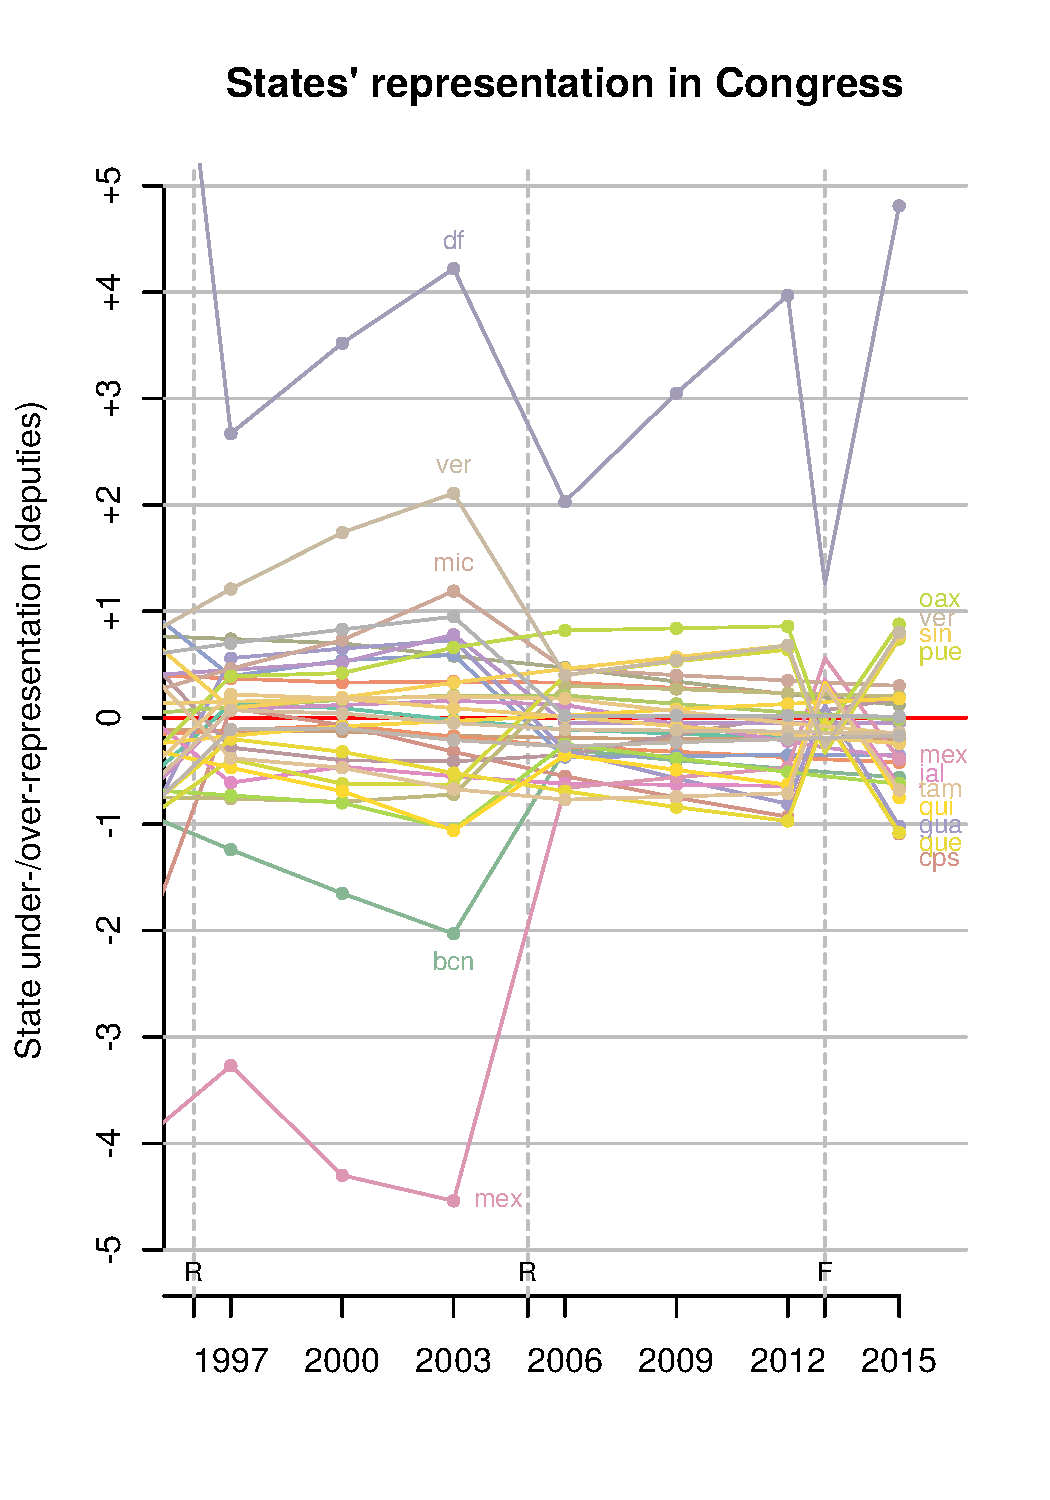
\includegraphics[width=.45\columnwidth]{statesUnderOverRep.pdf} & 
    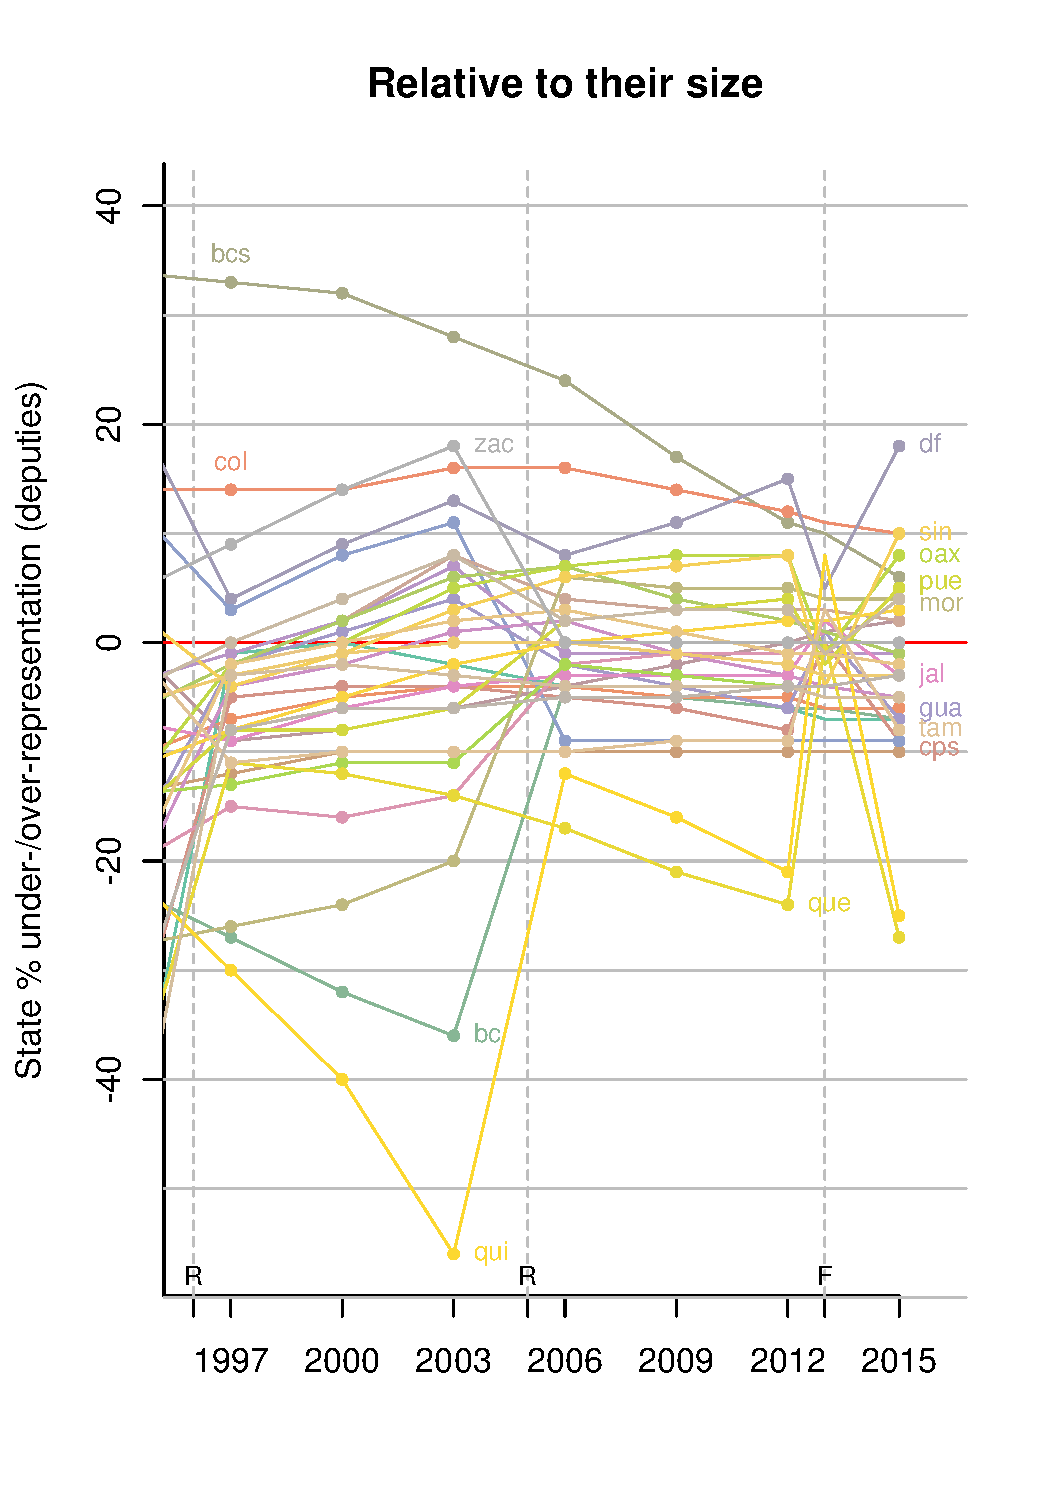
\includegraphics[width=.45\columnwidth]{statesUnderOverRep-rel.pdf} \\ 
  \end{tabular}
  \caption{Demography and state apportionment in Congress (lower chamber). Lines connect the seats that each state had relative to those it should have had on a population basis. Population projections from censuses used for this computation. Letters R in the horizontal axis indicate redistricting, letter F a redistricting failure (the effect that the proposed map would have had is reported on the dotted line). Source: prepared with data from \url{www.inegi.org.mx} and \url{www.ine.mx}.}\label{F:underOverRep}
\end{center}
\end{figure}

Figure \ref{F:underOverRep} summarizes states' congressional representation. In order to take creeping malapportionment into account, we projected each state's population at the time of a federal election between 1997 and 2015.\footnote{Projections up to 2010, inclusive, was by linear interpolation of census populations, and by linear extrapolation for 2012 and 2015. The years 1995 and 2005 had population counts, 2000 and 2010 had general censuses. The former collect much fewer respondent attributes than the latter, but report a population figure that we used.} With moving population estimates for election years, a time-series of states' fair share of congressional seats was then computed (i.e., time-varying $Q$s). Subtracting the actual number of seats apportioned to the state yields the state's over- or under-representation in election years. A state with perfect apportionment appears at zero in Figure \ref{F:underOverRep}. The slope in the line indicates deviations, downward for states losing relative weight in the lower chamber, positive for winners. The left panel reports this measure in absolute terms (so that $+3$ indicates a state with three deputies more than its fair share), the right panel relative to seats apportioned to the state ($+20$ indicates twenty percent more deputies than its fair share). Vertical dashed lines mark redistricting events (the ``F'' towards 2015 indicates a failed proposal to redistrict). 

Creeping malapportionment is manifest, points drifting between redistricting events. Since the first term of the subtraction is a real number and the second an integer, a fraction is bound to remain. Yet, upon redistricting, fractions in a well-apportioned systems should all be less than 1 quota in absolute value. The left panel shows that this is mostly the case, but exceptions are, and have always been present. The 2006 redistricting corrected the most egregious deviations from the ideal. The states of Baja North and of Mexico, with deficits of 2 and 4.5 deputies relative to population in 2003, respectively (deficits of 30 and less than 10 percent of the deputies they actually held), achieved near-parity in 2006. Over-represented Veracruz behaved near symmetrically to Baja in absolute terms (not relative). And a distortion strongly favoring the Federal District ($+4$ deputies) was somewhat attenuated in 2006, but never removed. 

The notorious case of the DF reveals that relying on obsolete population data is problematic. The constitution mandates the use of the census for redistricting, but has no obligation to redistrict as soon as it becomes available. As a consequence, drawing a new map for 2006 with data from the year 2000 injected a fair amount of creeping malapportionment into the new plan right at its inception. Compared to the 2000 census, our projected state population are off by 9.7 percent on average, with a standard deviation of 6.9 percent. Most states remained within the $[-1,1]$ range, but not the DF. With one extra year away from the reference census, the 1997 map had even less success achieving proper apportionment. One year closer to census makes a huge difference, as the abandoned map for 2015 reveals (although this is probably compounded with a less dynamic demography): the dotted vertical line at year 2013 reports how the new plan might have looked, have it been adopted. With this in mind, it is puzzling that the redistributive nature of apportionment has not pushed for the adoption of alternative methods. The seventeen states that were under-represented in 2006 jointly controlled a majority (162) of single-member districts; fourteen of them have always been below the red line indicating fair representation. 

%Persitent malapportionment is explained, in small part, by the allocation of two seats to small states. Relative over-representation of tiny Southern Baja and Colima was substantial, but only until recently. Population growth has made both worth their congressional seats. Yet relative over-representation remains substantial in migrant-worker-exporter Zacatecas up to 2003, and in the Federal District of late. Both states have lost population fast relative to the rest, and the system's design makes rapid demographic shifts slip away from grip. 

\subsection{Intra-state malapportionment}

% [Eric]: for broader paper, gerrymandering should also (mostly) be discussed here.

Unequally-sized districts are common practice in Mexico in spite of the automated application of clear quantitative redistricting criteria since 1997. In fact, Mexican parties in general, and IFE in particular, have been remarkably tolerant of this practice. This form of malapportionment is related, in some degree, to states' imbalanced apportionment in Congress, which perforce creates size differences across states' mean district sizes. But size inequality within states is also prevalent and substantial. 

Small deviations around a state's mean district population are unavoidable, especially as a map ages. But what constitutes significant deviation depends on the political context. Courts in the U.S.\ have struck down new district maps bearing less than 1\% differences without proper justification \citep{tuckerApportionment.1985}. Redistricting authorities generally view a \emph{de minimus} population deviations of as little as one or zero persons between congressional districts as desirable to inoculate against litigation. In stark contrast, IFE has considered deviations between 10\% (in 2006) and 15\% (in 1997 and 2015) above or below mean state district size perfectly normal \citep{lujambio.vives.2008,trelles.mtz.polygob2012}. If a pair of districts had populations exactly at the bounds of the $\pm15$ spread, the citizens at the bottom end would be worth one-third more in Congress than those at the top end. Surprisingly, no party has ever challenged this practice in Court. 

We inspect district population imbalance. As before, time-changing population estimates are behind this exercise. Following \citet{ansolabehere.gerber.snyderCourtRedis2002}, we measure a district's relative representation index as $RRI = \frac{1/\text{district size}}{300/\text{national population}} = \frac{Q}{\text{district size}}$, where the numerator is the number of congressional seats per person in the district and the denominator is the average number of congressional seats per person nationwide (300 is the number of congressional seats).\footnote{Ansolabehere et al.'s $RRI$s were devised to measure how well are represented counties (some of which have several districts) in U.S.\ state assemblies. In our case, all units are a whole districts.} Since the denominator represents the inverse of the apportionment quota $Q$, the second equality is a convenient algebraic transformation. A district with unity index value has representation matching the `one person, one vote' ideal perfectly. Values above one indicate over-representation, values below one under-representation, and the measure is continous. An example shows how the index is interpreted. The size of the 3rd district of Aguascalientes in 2012 was about 306,000 inhabitants, and the (projected) quota about 387,000, so the district in question had 26 percent more representation than the national average, for an index value of 1.26. As before, we used population projections to compute $RRI$s.\footnote{Census data reported at the electoral \emph{secci\'on} level (used to aggregate district populations in two maps) are available since 2005 only. We projected the 2005--2010 changes to 2006 and 2015 for this exercise. Since many districts are made of full municipalities, we could use that unit to interpolate all the way to 1997.} 

Redistricting automation should make districts within states tend towards zero malapportionment. The electoral bureaucracy claims that population balance is an important criterion, and assigns it a nominal weight higher than all other criteria \citep{altman.magar.mcd.trelles2014apsa}. However, in practice the system allows population balance to easily be trumped by other criteria.\footnote{The other criteria are the preservation of municipal boundaries, travel times within the district, and district compactness. All are achieved by exploiting tolerated population leeway.} $RRI$s can also be expressed relative to state populations by replacing the denominator with the average number of congressional seats per person in the district's parent state (i.e., the number of seats in the state over the state's population). With three seats apportioned to the state of Aguascalientes and a total population of about 1,200,000, the 3rd district had 33 percent more representation than the state average, for an index value of 1.33. This is instructive to inspect within-state representation. The percentiles corresponding to state $RRI$s equal to .85 and 1.15 (the bounds of IFE's $\pm15$ percent tolerance range) in 2006 were 6 and 89, respectively, implying that $6+100-89=17$ percent of districts were outside the range relative to the average state population. That was the map's inaugural year. By 2012, as many as 27 percent districts were off the population tolerance range, and by 2015 one third will be. Drawing equal-sized district boundaries with old population data is no easy task, and distorts representation within states over and above between-state imbalances.  

% USED CODE IN RED.R TO DO THIS PLOT
\begin{figure}
\begin{center}
    % 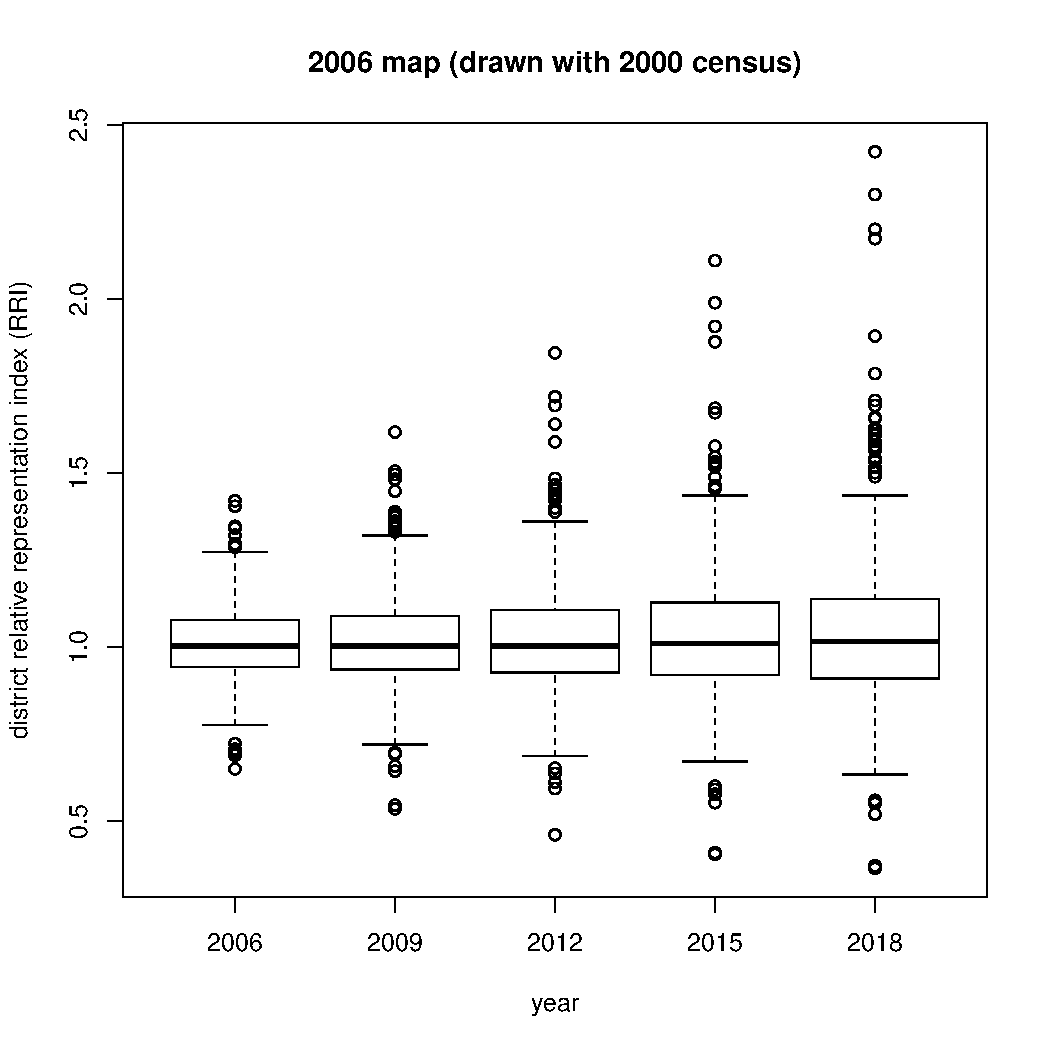
\includegraphics[width=.65\columnwidth]{rris0618d0.pdf} \\ 
    % 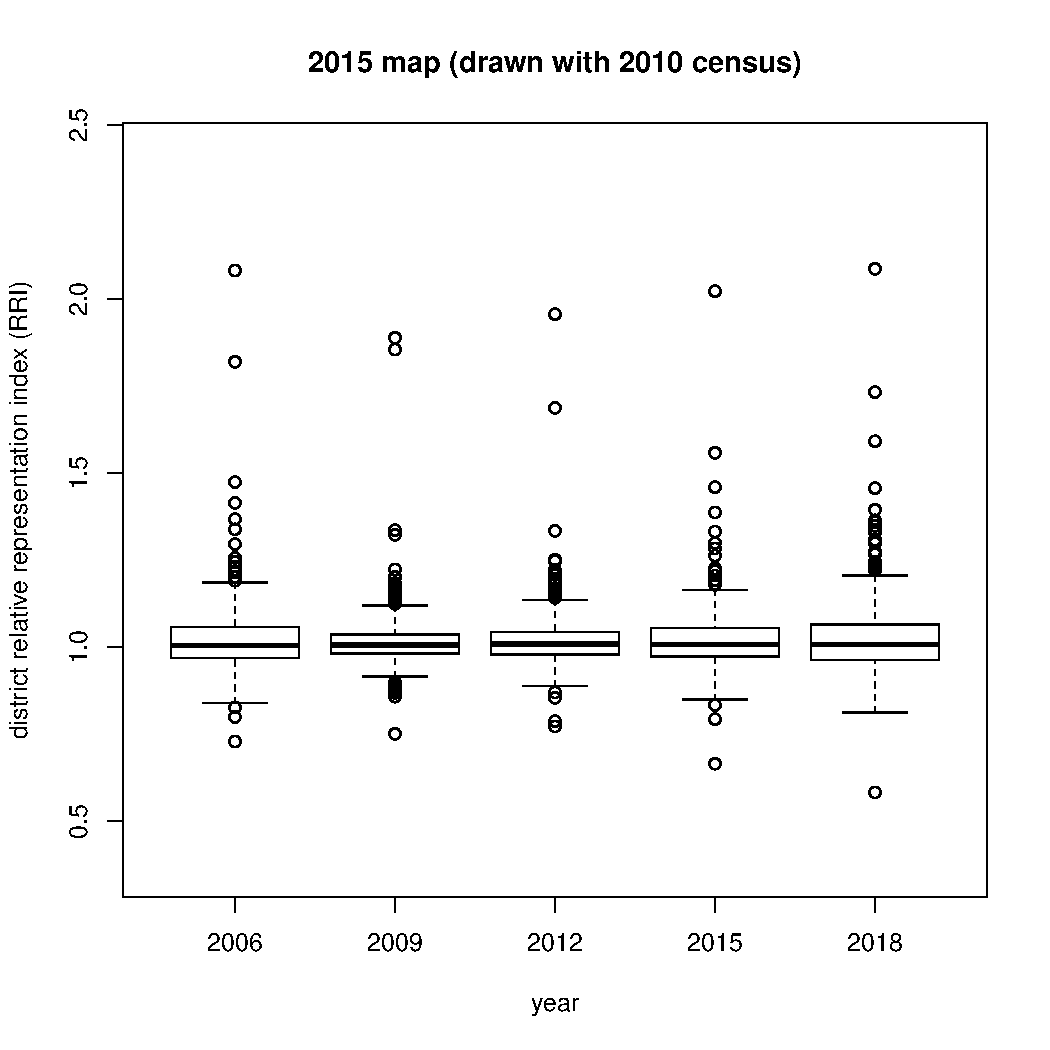
\includegraphics[width=.65\columnwidth]{rris0618d3.pdf}  
\begin{tabular}{cc}
    (a)&(b)\\
    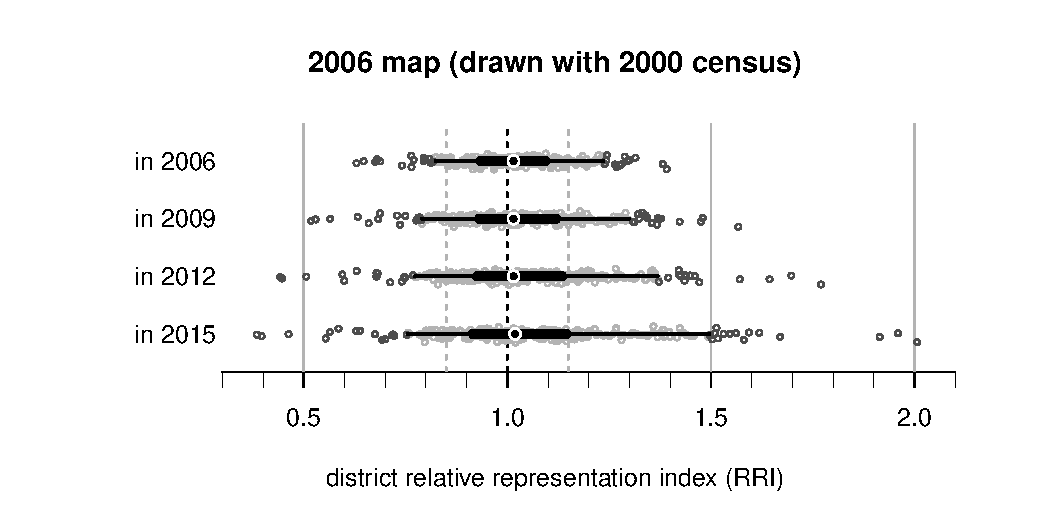
\includegraphics[width=.5\columnwidth]{rrin0615d0.pdf}&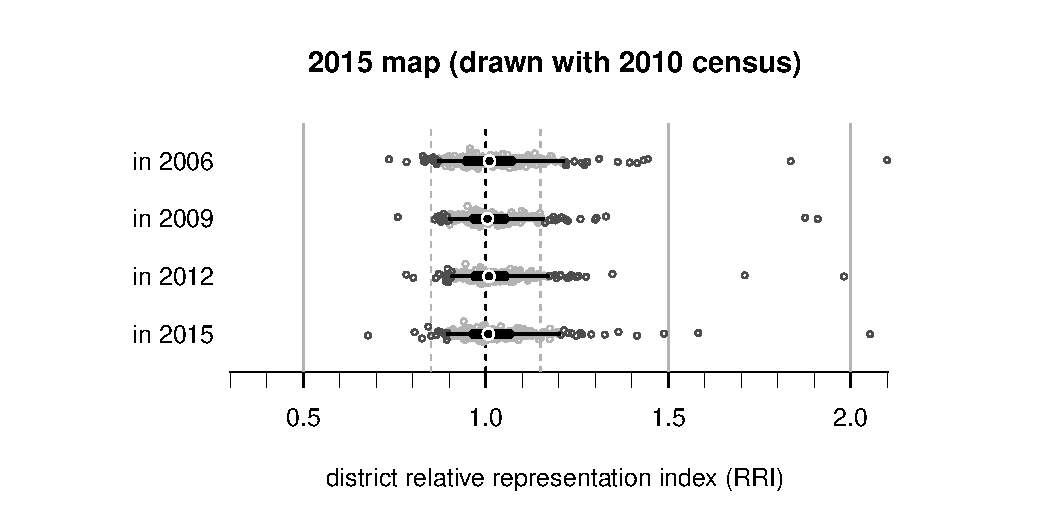
\includegraphics[width=.5\columnwidth]{rrin0615d3.pdf}
\end{tabular}
\caption{Representation in four elections and two maps. Panel (a) portrays the 2006 map (status quo), panel (b) the hypothetical 2015 map. Finer horizontal lines connect the 5th and 95th percentiles, thicker lines the quartiles, and white circles indicate the median. Points represent districts, hollow for outliers.}\label{F:malapp}
\end{center}
\end{figure}

Figure \ref{F:malapp} returns to $RRI$s computed with the national average. Nationwide, the $\pm15$ band has been substantively surpassed. Plots summarize the distribution of citizen representation as population has fluctuated. Consider the top plot first. Each point represents one district. The fine horizontal line connects the $RRI$ values corresponding to the 5th and 95th percentiles---both well outside the tolerance band, represented by dashed gray lines, since the map's inauguration. The thick horizontal line is the inter-quartile range, nearly covering the full tolerance band by 2015---implying that soon half the districts will be off-range! For the 2015 midterm congressional election, citizens in the plot's right-most districts (in central Monterrey and two in battered Ju\'arez) will be worth \emph{four times more} in Congress than citizens in the left-most districts (one each in suburban Monterrey and Mexico City, the other in Canc\'un). Politically, citizens at one quartile will be nearly worth twice as much as those at the other quartile. 

The bottom plot offers a counterfactual, adopting the hypothetical map that was drawn towards the 2015 election but abandoned. It is quite clear that, even if outliers remain in its inauguration, the hypothetical map would have represented Mexicans much better than the status quo (note the narrower horizontal lines). Taking the mental experiment further, it is possible to aggregate section-level population projections for 2009 into the hypothetical map to assess it performance in the year closest to the census on which the map was prepared. Like fish, demographic information must be fresh: all but a handful of hypothetical districts in that year are within the $\pm15$ band. 

The evidence is unambiguous: malapportionment in Mexico is systematic and substantial.\footnote{The comparative survey by \citet{snyder.samuelsMalapp2004} ranked Mexico among well-apportioned cases. The measure reported is for the 1997 map, but no guidance is offered about the population figures used in denominators. We suspect reliance---as IFE did then and still does now---on raw 1990 census data, severely underestimating malapportionment.} %How much it translates into party bias is the subject to which we now turn attention. 

\section{Expectations}

On paper, IFE is an autonomous, non-partisan election regulator. Members of its Council-General are thoroughly vetted and recruited from among professionals without party affiliation and admitted after winning consensual endorsement in the Chamber of Deputies. Once in office, councilors enjoy secure tenure. Their budget, which includes generous public financing for political parties and their electoral campaigns, is subject to few political whims. Yet closer inspection of the structure and process reveals how the Council-General is, in practice, a power-sharing agent of the major congressional parties \citep{estevez.magar.rosas.2008}. The systematic partisan segmentation of the Council-General is quite conclusive evidence that major-party influence in electoral regulation is unremitting. 

If the Council-General acts as an agent of the major parties, then one should observe the following: 

\begin{enumerate}

\item When a map is adopted, districts have no bias favoring one major party relative to another. If a new map has bias, it must be against minor parties relative to major ones. 

\item As maps age and district populations drift away from census relative levels, party bias (malapportionment-based) can creep in. Party bias should therefore grow with each failure to redistrict. 

\item There is no partisan gerrymandering. Distributional-based advantage for a party one year will be compensated by distributional-based handicap in other years, changes from one year to next according to parties' electoral fortunes

\end{enumerate}

%With such setting, the possibility that districts are granting undue advantage to the PRI merits closer inspection. A priori, reasons to suspect IFE of cooking districts to favor one party or another are lacking. 

%That those who draw the district lines can distort a fundamental link of the democratic process is well established in the literature \citep{altman.mcdonald2011bard,cox.katz.2002,engstrom2006redisttrictApsr,rossiter.etal.1997,otero.2003}. Has the insidious gerrymandering reared its ugly head in Mexico? 

% Major parties, after all, permanently influence the election regulator, ambition counteracting ambition \citep{estevez.magar.rosas.2008}. 




% \section{Redistricting since 1997}

% The original 300 SMD districts map adopted in 1979 was redrawn in 1997, coinciding with the first free and fair congressional election \citep{lujambio.vives.2008}. Redistricting occurred again in 2006, and was ready for adoption, but postponed, in 2015. The PR tier is elected in five forty-member districts that have also changed in recent decades \citep{palacios.tiradoCircPluris2009}. Since PR boundary lines were not redrawn in the most recent redistricting proposal of 2015---on which analysis concentrates---we leave them out of the analysis. Future inspections of previous redistricting events would do well to take them into account. From now on in this paper, by seats/districts we always refer to the SMD kind. 

% We name the distinct maps by years. We stick to the convention of using not the date when boundaries were actually redrawn and accepted, but that of the first election the map was (or would have been) used. Thus, there is a ``1979 map'' actually drawn in 1978, a ``1997 map'' drawn in 1996, a ``2006 map'' drawn in 2004--05, and a ``2015 map'' drawn in 2013, but never used. Machine-assisted mapping has been in use since 1997. Details have changed, but the broad lines have not \citep{trelles.mtz.polygob2012}. We describe the three major stages of the redistricting process: the apportionment of seats to states; the design of an optimization algorithm; and the strategic assessment of computer-generated district blueprints by technocrats with the active, but limited involvement of political parties. 

% \textbf{Apportionment}. Redistricting starts by redistributing a fixed number of seats among the 32 states.\footnote{The Federal District, where Mexico City resides, is not a state proper, but is treated as one for the purpose of apportionment and redistricting.} Restrictions, reminiscent of the U.S., apply at this stage: no state may have fewer than two seats; the sole redistributive criterion above that minimum is state population; and no district may cross state boundaries. 

% \textbf{Optimization}. This stage adopts a set of desiderata for a new map drawn from the base geography. A technical committee, appointed by IFE's Council General, is in charge of optimization and proposing a map for assessment. The formal ``cost function'' devised for the 2015 map included four criteria: population balance (given a relative weight of .4 in the linear combination), municipal boundary preservation (weight .3), travelling times inside the district (weight .2), and district compactness (weight .1). Trade-offs between them would inevitably step in as district boundaries are calibrated. Assisted with computers, the process made marginal changes, repeatedly reassigning geographical blocks between districts, while systematically checking the cost. Through iteration with different random seeds, cost-minimizing district maps for each state were generated.\footnote{More refined optimization algorithms have been used in each redistricting round. The 2015 algorithm, described here, replaced a method of simulated annealing used in 2006.} The building blocks are more than 66 thousand \emph{secciones electorales} into which the Mexican territory is subdivided. \emph{Secciones} are analogous to U.S.\ census tracts, but somewhat bigger. Median \emph{secci\'on} population in the 2010 census was 1,280 persons, with a maximum at 79,232. 

% Restrictions also apply at this stage: contiguity is a must, as no district can have exclaves; and guarantees for minority representation must be considered, not partitioning \emph{municipios} (the lowest elected offices, similar to counties in the U.S.) with sizeable indigenous populations. IFE would tolerate population imbalance of up to 15\% from mean district size (the threshold was 10\% in 2006), and even deviations beyond that threshold with proper ``technical justification'' \citep{ife.acuerdoRedis2013}. The last item is of much importance for our argument, and elaborate it further below.

% \textbf{Assessment}. In this stage, that we study elsewhere \citep{altman.magar.mcd.trelles2014apsa}, the technical committee, party representatives, and the Council General interact. The map proposal is distributed to the parties for analysis and discussion. Parties suggest modifications to district boundaries, which the technical committee accepts if they improve the score from the optimization algorithm. Revisions adopted become the starting point for a second, and final round of observations/amendments. The final plan is then presented to the Council General for formal approval. It is at this final stage that the 2015 redistricting was abandoned. The Council General opted to put the process on hold until the details of an ongoing major electoral reform in Congress became known. As a consequence, the 2015 midterm election will be held with significantly outdated districts. 


\section{Methods}

%This section estimates majority and party effects in the proposed districts and the status quo. Majority effects are huge, partisan effects negligible. 

A multiparty and estimable version of equation \ref{E:kingBi} \citep{king.1990elRespBiasMultiparty} establishes that party $p$'s ($p=1,2,\ldots,P$) expected seat share is 

\begin{equation}\label{E:kingMulti}
 E(s_p) = \frac{e^{\lambda_p} * v_p^\rho}{\sum_{q=1}^{P} e^{\lambda_q} * v_q^\rho}
\end{equation}

\noindent with data and parameters now indexed to identify the parties \citep[another is][]{calvo.micozzi.govReform.2005}. Setting $\lambda_2 = 0$ restricts the remainder $\lambda_{p \neq 2}$ to express party bias with relation to the PRI's ($p=2$ in the dataset). This is convenient. Party bias in two-party competition is asymmetry in a vote--seat curve centered on $v=.5$ (see Figure \ref{F:lambdaRhoEx}). There is no reason to expect a .5-centered curve in multiparty competition, nor is it a priori evident what vote should serve as center point, a difficulty towards expressing the party bias estimate $\hat{\lambda}_p$ as a percentage points advantage or handicap for party $p$ in the votes-to-seats conversion. Finding $\lambda_{p \neq 2}<0$ would be evidence of PRI-favoring bias. %And expressing party bias relative to the PRI in particular eases assessment of the presumption of PRI-favoring bias: if present, $\lambda_{p \neq 2}<0$ would result.

A common estimation strategy relies on a time-series of election returns. \citet{marquez2014biasBlog} does this using votes and seats won over two decades, uncovering a degree of responsivity characteristic of plurality systems and substantive party bias against the PAN. Multi-election studies offer more data points for estimation, but inevitably sacrifice comparability, especially over the longer haul \citep{jackmanMeasuringBias1994}. It is district-level margins, after all, that determine seats won, and two district margin distributions could conceivably yield very similar national vote aggregates but quite different seat shares---a classical problem of over-determination. Single-election studies are therefore preferable \citep{niemi.fett1986swing}, and procedures to multiply data points desirable. Dis-aggregation is one approach: reliance on state-level congressional election votes and seats, instead of standard national-level aggregates, offers a 32-fold hike in data points (patent between panels in Figure \ref{F:seatsVotes}). But it treats state party systems as the national, and has pitfalls similar to longitudinal multiplication. %\citep[][ attempt this approach]{magar.altman.mcd.trelles2014uh}. %One obvious disadvantage of the approach is that states have few districts (9.4 on average), and this will amplify the system's responsiveness \citep{taagepera.CubeLaw.1973}. It should not, however, affect estimates of party bias, our substantive interest. 

The multiplication strategy adopted here, inspired by \citet{linzerSeatVoteElasticity2012} and explored by \citet{marquez2014mixSwingBlog}, relies on Monte Carlo simulation instead.\footnote{We did not pursue Linzer's swing ratios. The relation of that quantity with the notion of party bias adopted here is straightforward in balanced two-party competition \citep[see][:410]{linzerSeatVoteElasticity2012}, but not when multiple parties compete. We therefore followed his method part of the way, borrowing his code to generate hypothetical national party vote and seat pairs, but fitting our model on those.} Towards this goal, a probability density of national party vote returns is approximated from observed district outcomes with a finite mixture model. FMMs work with district-level data, assuming sub-populations with known distributions are present (e.g., some districts where party 1 vote grows at the expense of party 2's, others where they grow together) but information to match districts to sub-populations is unavailable. A mix of the known distributions describes the unknown distribution. Repeated draws of hypothetical district outcomes from the mix reflect variation in the sources of party bias: in district size, in turnout, and in vote choice (the FMM was fed with this information); and aggregating them nationwide yields a large sample of vote--seat simulations that are supported by the data.\footnote{An online appendix describing the multiplication procedure in detail, and with commented code extending Linzer's procedure will be posted upon publication.} 

(**s:v plots of each election with data and sims in gray, to discuss here?**) One limitation is that the mixture offers reliable simulations only near parties' observed vote shares (about $\pm10$ percent), and inference at extreme counterfactuals is driven by the vote--seat model's parametric assumptions (Equation \ref{E:kingMulti}). But this complication arises in every attempt to fit vote--seat curves with a limited number of data points from an empirical referent. And the approach is very attractive, allowing analysis of 100 simulated national votes--seats points by party for each federal election in the period.  

%The actual district structure remained constant throughout the 2006, 2009, and 2012 federal deputies elections studied here. %And it takes advantage in the variation of state party systems (this draft fails to take full advantage of this variance, but this could be exploited further). 

%We proceed with state-by-state breakdowns over much a shorter span (2006, 2009, and 2012). Doing so, much higher responsivity (owing to fewer districts, 9 by state on average) is uncovered, but no apparent party bias in neither the 2006 map nor 2015 proposals. 

\section{Data}

The data section should briefly discuss the data sources, their caveats, and how they were recoded/matched/integrated by us---and provide a citation to a replication file (or at least a placeholder). 


\section{Results}

% [Micah]: Section 3 states very clearly three expected observations of the power-sharing hypothesis -- we should note clearly the evidence for each

\subsection{Raw party bias}

The method of estimation is MCMC \citep{jackman.2000}.\footnote{Three chains were iterated 10 thousand times, taking every fiftieth observation of the last 5 thousand to sample the posterior distribution. The Gelman--Hill $\hat{R} \approx 1$ \citep{gelman.hill.2007}, evidence that the chains had reached a steady state. Convergence was also inspected visually in chain traceplots of each of the model's parameters. Estimation performed with open-source software: JAGS \citep{jags.cite}, implemented in R \citep{r.cite} with library R2jags \citep{r.r2jags}. Data and commented code to replicate the analysis will be posted on-line upon publication.} To obtain the GKB separate party bias sources, equation \ref{E:kingMulti} was estimated as it appears, then replacing $v_p$ by $\bar{v}_p$, then by $\bar{w}_p$. Single-election estimates were obtained for four congressional elections between 2003 and 2012. 

\begin{figure}
\begin{center}
  % \begin{tabular}{cc}
  %   (a) & (b) \\
  %   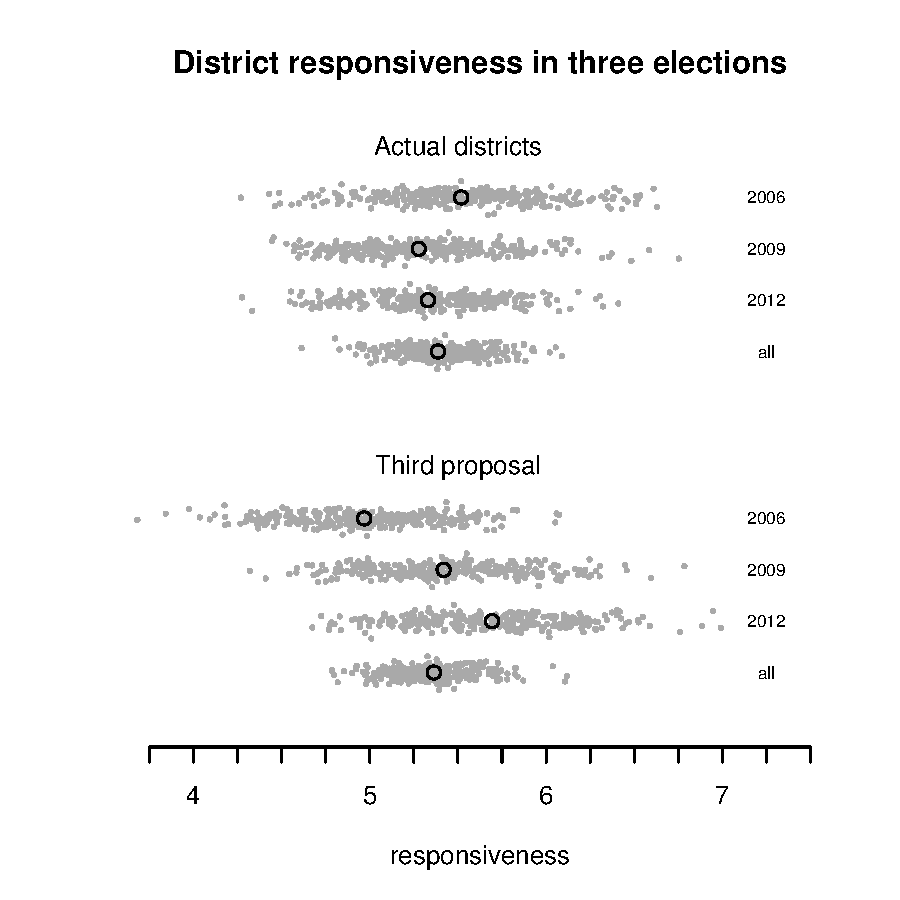
\includegraphics[width=.45\columnwidth]{resp200612s0s3.pdf} &
  %   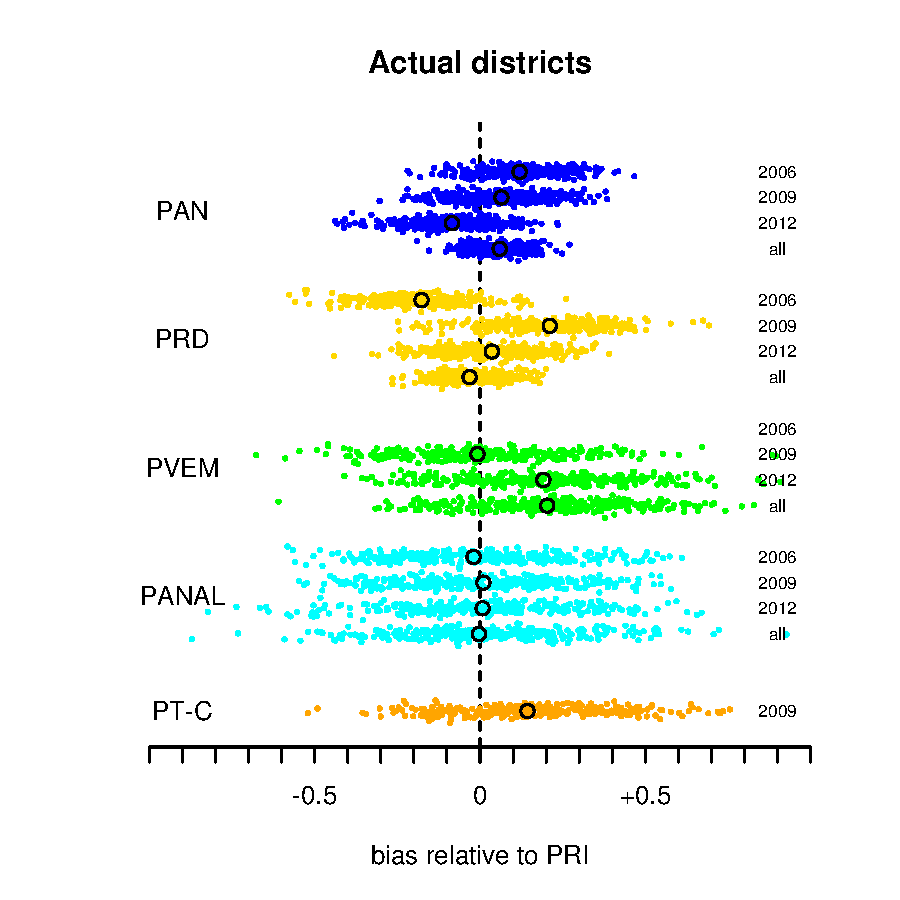
\includegraphics[width=.45\columnwidth]{bias200612s0.pdf} \\
  %   (c) & (d) \\
  %   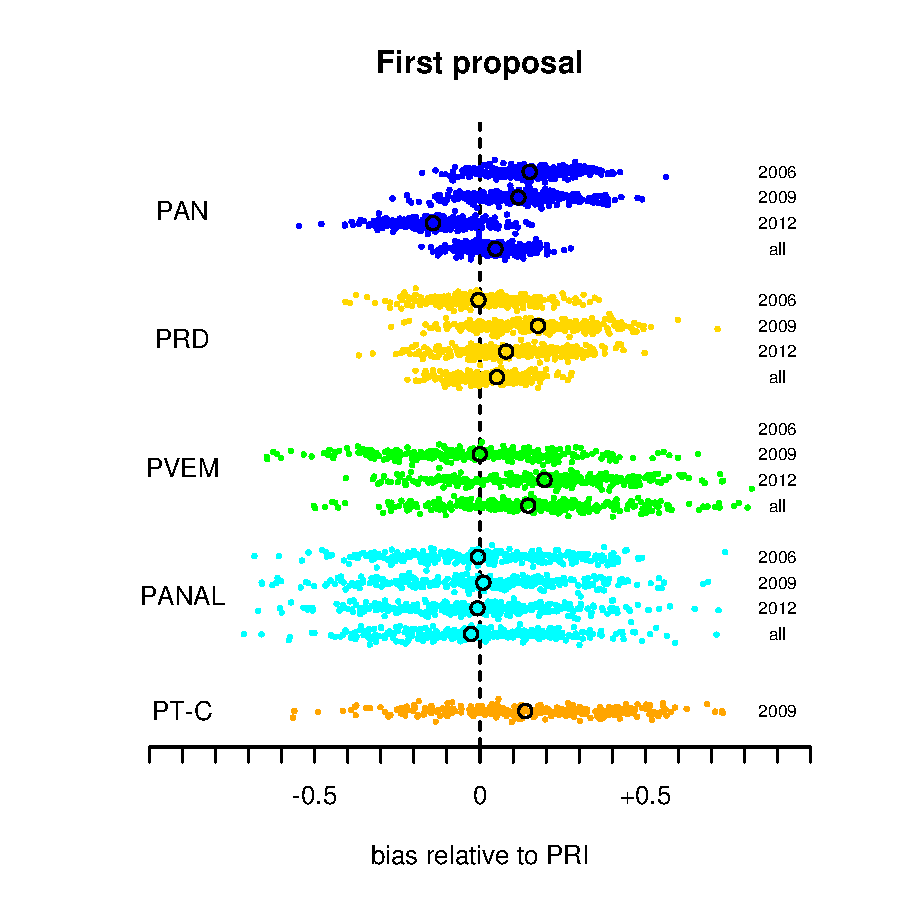
\includegraphics[width=.45\columnwidth]{bias200612s1.pdf} &
  %   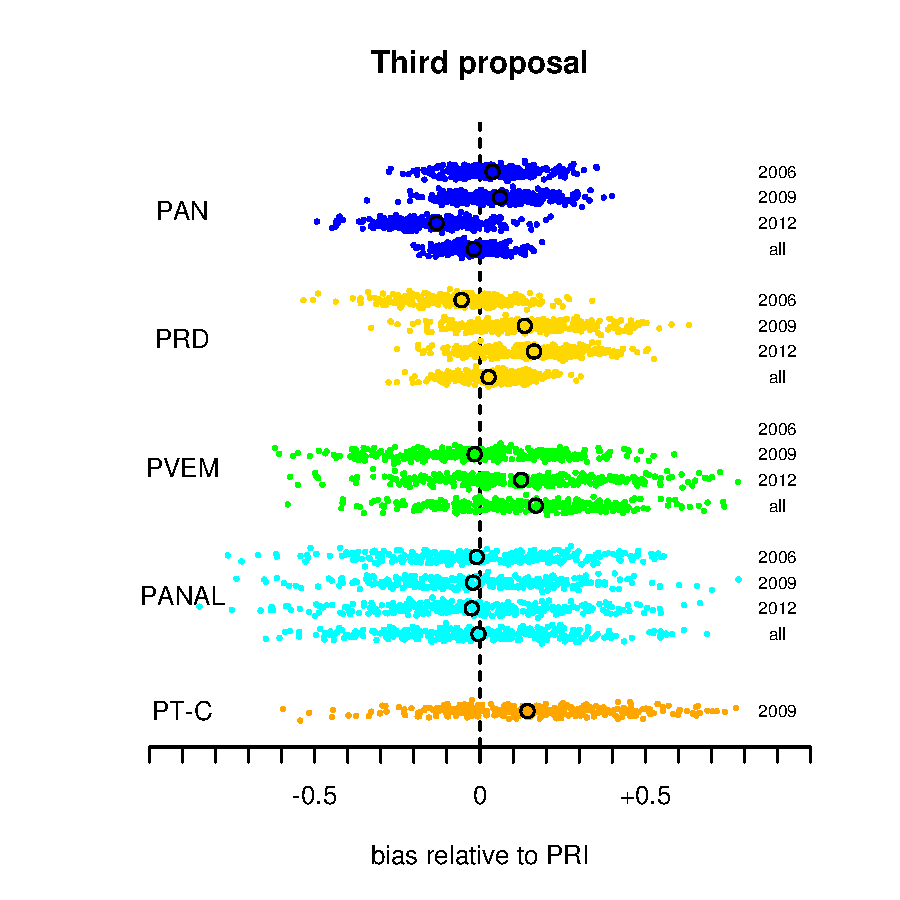
\includegraphics[width=.45\columnwidth]{bias200612s3.pdf} 
  % \end{tabular}
  % \begin{tabular}{cc}
  %   \mc{2}{c}{(a)} \\
  %   \mc{2}{c}{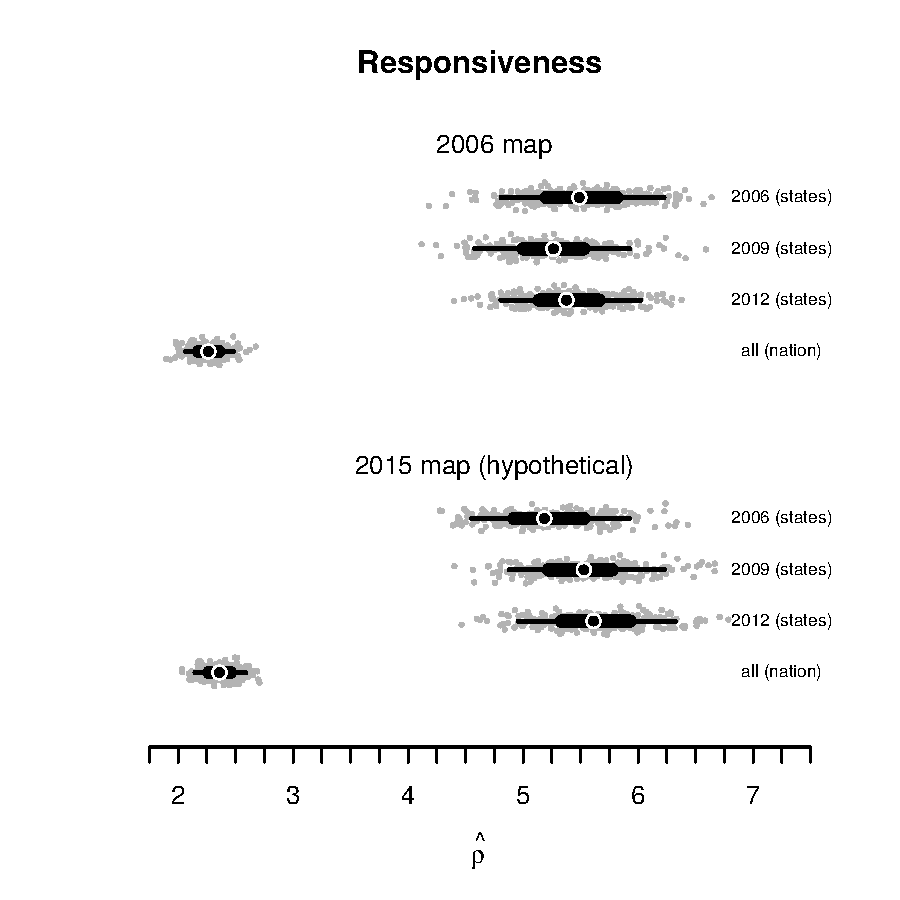
\includegraphics[width=.5\columnwidth]{resp200612s0s3R.pdf}} \\
  %   (b) & (c) \\
  %   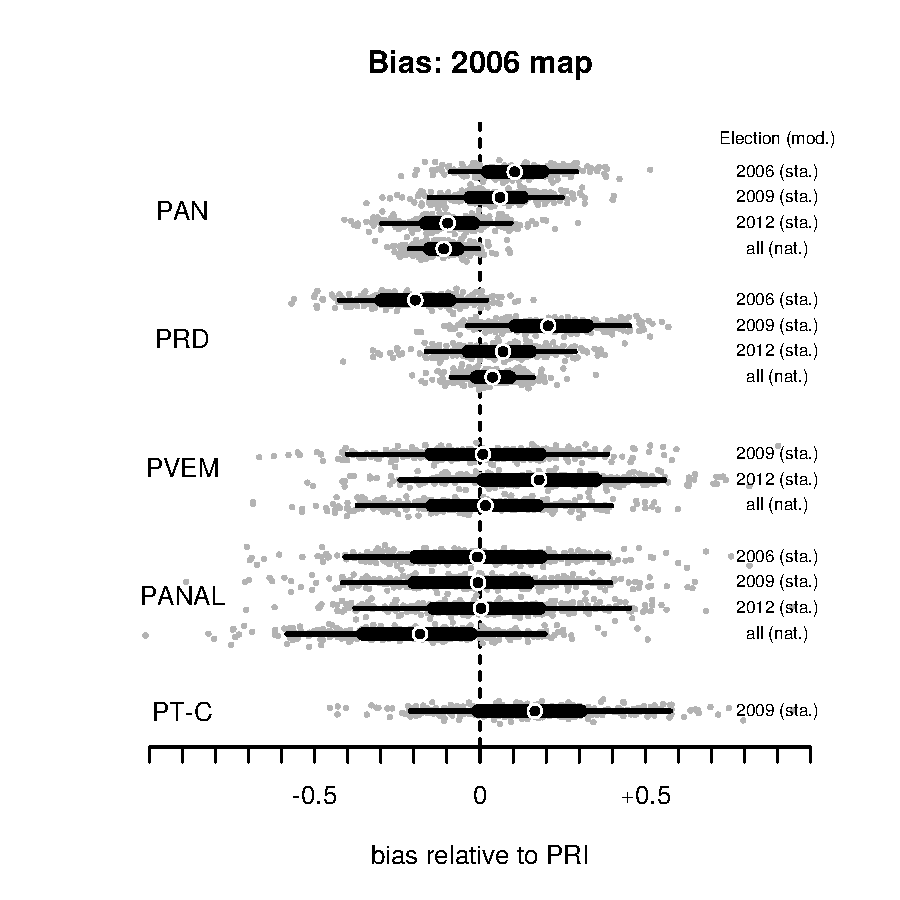
\includegraphics[width=.5\columnwidth]{bias200612s0R.pdf} &
  %   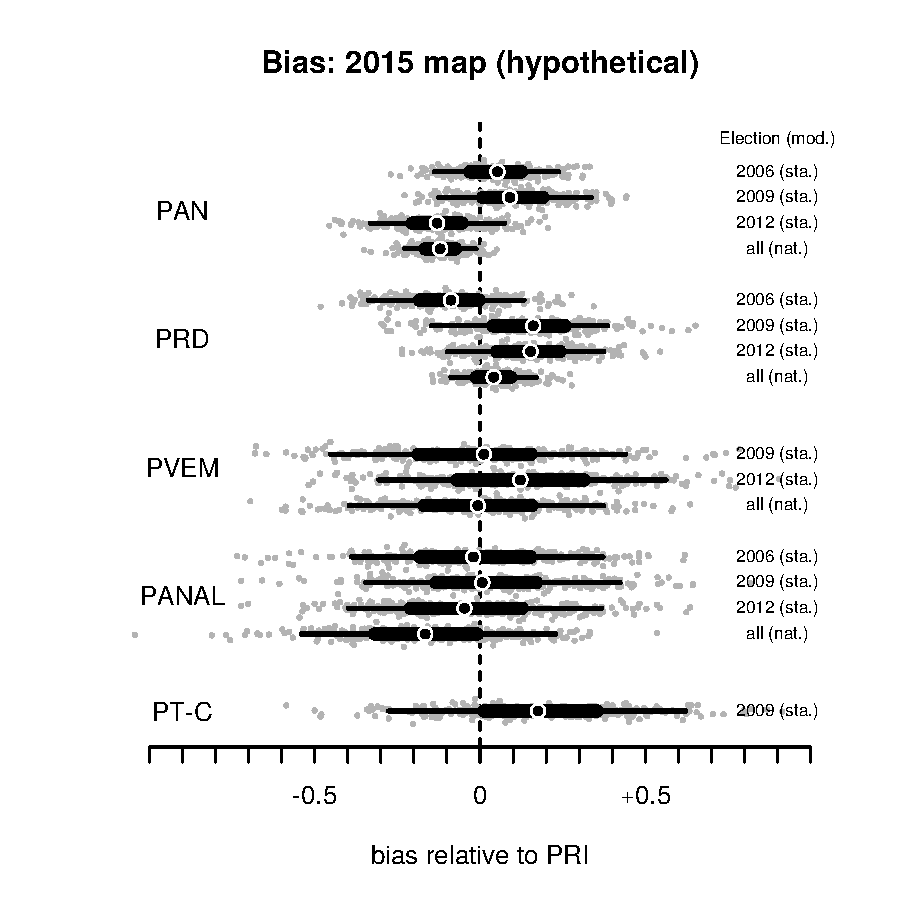
\includegraphics[width=.5\columnwidth]{bias200612s3R.pdf} 
  % \end{tabular}
    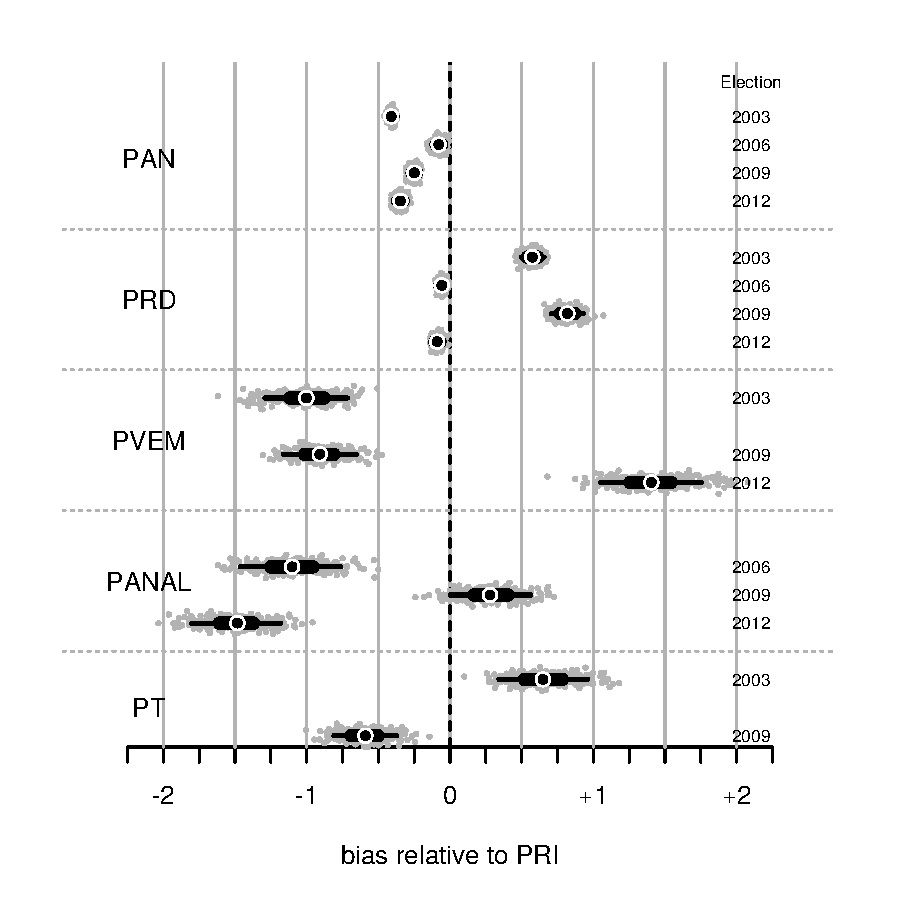
\includegraphics[width=.9\columnwidth]{bias200612d0R.pdf} 
  \caption{Raw party bias in four elections. The plot describes the posterior samples (small gray points) of estimated parameters $\hat{\lambda_p}$ for five parties. Some parties did not run in some years. Finer horizontal black lines connect the 5th and 95th percentile values of the posterior sample, thicker lines the quartiles, and white circles indicate the median value.}\label{F:posterior_s0s3}
\end{center}
\end{figure}

The responsiveness parameter, of secondary interest here, serves to assess the general model fit. Judging the 90-percent Bayesian confidence intervals (i.e., the 5th to 95th percentile range of $\hat{\rho}$'s posterior sample) reveals sizable shifts in the estimate between congressional elections: from a low of $[2.2,2.4]$ in 2012 to a high of $[2.6,3]$ in 2006. (Is inter-election drift in $\rho$ mentioned in the literature?) The large-party premium of recent Mexican plurality congressional races is about one-sixth smaller than the power of the putative cube law of plurality elections \citep{taagepera.CubeLaw.1973}. 

Raw party bias results (i.e., the $\lambda_p$ parameters estimated using $v_p$) bear more direct interest. Figure \ref{F:posterior_s0s3} reports summaries of the posterior sample for different parties. The absence of the PRI is due to its choice are reference to express party bias measures. Several patterns are noteworthy. Estimate precision (i.e., how concentrated the posterior sample's cloud appears) is consistently lower for minor parties. Among the major ones, the PAN's estimates excel, variation around the median posterior value (taken as the point estimate) nearly indistinguishable every year. The PRD's generally precise estimates are slightly less so in midterm elections (2003 and 2009) than in presidential election years. And the size and polarity of estimates reveal important party differences. The PAN experienced negative, albeit small bias vis-\`a-vis the PRI in every year observed. Leaving aside the question of how meaningful the estimated quantities---we analyze swing ratios below with this object---the near exception was 2006, when the cloud nearly overlaps with the zero's vertical line and the estimate is tiny. 

In stark contrast, the left experienced favorable and substantive bias relative to the PRI in some years but not in others. In this respect, bias for the left is a mirror image of its electoral fortunes: it vanished when its candidates for Congress rode L\'opez Obrador's presidential campaign coattails (the party's national congressional vote was 30 percent on average in 2006 and 2012), but materialized otherwise (when vote averaged 16 percent).\footnote{Parties' national vote shares in the period were: \begin{tabular}{rrrrrr} Year & PAN & PRI & PRD & Green & PANAL \\ \hline 2003 & .32 & .38 & .18 & .04 & --- \\ 2006 & .34 & .28 & .31 & --- & .05 \\ 2009 & .29 & .40 & .14 & .06 & .04 \\ 2012 & .27 & .38 & .28 & .02 & .04 \\ \end{tabular}} In spite of losing about half of its electoral support, the PRD converted votes into seats much more efficiently than either other major party in midterm election years. Whether this was due to winning smaller districts or lower-turnout districts we answer next.

\subsection{Components of party bias}

Table \ref{T:GKBbreakdown} breaks down raw party bias into GKB's additive components: the distributive, the turnout, and the malapportionment bases. Ignore the right column for now. Relative bias estimates for the PAN, the PRD, and a selected minor party vis-\`a-vis the PRI are included. The minor party in 2006, 2009, and 2012 is the Green, and in 2006 the PANAL (close to the teachers' union). The Green ran in pre-election coalition with the PRI in a changing number of districts every year---one-fifth of all in 2009, one-third in 2003, two-thirds in 2012, and in all districts in 2006---hence the choice of another minor party to report that year. Numbers in parentheses report the share of the posterior sample that has a sign opposite to the one reported, and therefore serves as a test of the estimate's statistical significance (the probability that the estimate's sign is wrong). %As a result, the party fielded candidates and received a vote share in less than all districts. 

% %% Reports state-agg in 3 yrs and in 2 maps
% \begin{table}
% \centering
% %\newcolumntype{d}[1]{D{.}{.}{#1}} % D column with 1 decimal spaces default, usage d{2} for two spaces
% \newcolumntype{d}{D{.}{.}{2}} % D column with space for 2 decimal spaces
% \begin{tabular}{lddd|ddd}
%               & \mc{3}{c|}{2006 map} &  \mc{3}{c}{2015 map (hypothetical)} \\
% party bias    &  \mc{1}{c}{\textsc{pan}--\textsc{pri}}  &  \mc{1}{c}{\textsc{prd}--\textsc{pri}} &  \mc{1}{c|}{\textsc{pan}--\textsc{prd}}  & \mc{1}{c}{\textsc{pan}--\textsc{pri}}  &  \mc{1}{c}{\textsc{prd}--\textsc{pri}} &  \mc{1}{c}{\textsc{pan}--\textsc{prd}} \\  \hline
% \mc{7}{l}{\textbf{~2006 election (states)}}   \\
% raw           &   0.10 &  -0.20 &   0.30 &   0.05 &  -0.09 &   0.14 \\
% distrib.      &   0.18 &  -0.19 &   0.37 &   0.14 &  -0.09 &   0.23 \\
% turnout       &  -0.10 &  -0.01 &  -0.09 &  -0.06 &   0.00 &  -0.06 \\
% malapp.       &   0.02 &   0.00 &   0.02 &  -0.03 &   0.00 &  -0.03 \\
% \mc{7}{l}{\textbf{~2009 election (states)}}  \\
% raw           &   0.06 &   0.21 &  -0.15 &   0.09 &   0.16 &  -0.07 \\
% distrib.      &   0.09 &   0.16 &  -0.07 &   0.13 &   0.12 &   0.01 \\
% turnout       &  -0.04 &   0.05 &  -0.09 &  -0.03 &   0.02 &  -0.05 \\
% malapp.       &   0.02 &   0.00 &   0.02 &  -0.01 &   0.02 &  -0.03 \\
% \mc{7}{l}{\textbf{~2012 election (states)}}  \\
% raw           &  -0.10 &   0.07 &  -0.17 &  -0.13 &   0.15 &  -0.28 \\
% distrib.      &  -0.09 &   0.02 &  -0.11 &  -0.07 &   0.14 &  -0.21 \\
% turnout       &  -0.04 &   0.03 &  -0.07 &  -0.05 &   0.00 &  -0.05 \\
% malapp.       &   0.04 &   0.01 &   0.03 &  -0.01 &   0.02 &  -0.03 \\
% \mc{7}{l}{\textbf{~All elections (nation)}}    \\
% raw           &  -0.11 &   0.04 &  -0.15 &  -0.12 &   0.04 &  -0.16 \\
% distrib.      &  -0.04 &   0.13 &  -0.17 &  -0.04 &   0.17 &  -0.21 \\
% turnout       &  -0.07 &  -0.13 &   0.06 &  -0.08 &  -0.13 &   0.05 \\
% malapp.       &   0.00 &   0.05 &  -0.05 &   0.00 &   0.00 &   0.00 \\ \hline
% \end{tabular}
% \caption{Relative major-party bias. Single-election entries report raw bias and its additive components from parameters estimated with the state aggregates model. Multi-election bias estimated with the national aggregates model.}
% \end{table}

% %% reports state-agg and MC side-to-side
% \begin{table}
% \centering
% %\newcolumntype{d}[1]{D{.}{.}{#1}} % D column with 1 decimal spaces default, usage d{2} for two spaces
% \newcolumntype{d}{D{.}{.}{2}} % D column with space for 2 decimal spaces
% \begin{tabular}{lddd|ddd}
%               & \mc{3}{c|}{state-aggregates} &  \mc{3}{c}{MC simulations} \\
% party bias    &  \mc{1}{c}{\textsc{pan}--\textsc{pri}}  &  \mc{1}{c}{\textsc{prd}--\textsc{pri}} &  \mc{1}{c|}{\textsc{pan}--\textsc{prd}}  & \mc{1}{c}{\textsc{pan}--\textsc{pri}}  &  \mc{1}{c}{\textsc{prd}--\textsc{pri}} &  \mc{1}{c}{\textsc{pan}--\textsc{prd}} \\  \hline
% \mc{7}{l}{\textbf{~2003 election}}   \\
% raw           &        &        &        &  -0.37 &  0.72 & -1.09  \\
% distrib.      &        &        &        &  -0.09 &  0.69 & -0.78  \\
% turnout       &        &        &        &  -0.26 & -0.11 & -0.15  \\
% malapp.       &        &        &        &  -0.01 &  0.14 & -0.15  \\
% \mc{7}{l}{\textbf{~2006 election (states)}}                        \\
% raw           &   0.10 &  -0.20 &   0.30 &  -0.08 & -0.06 & -0.02  \\ 
% distrib.      &   0.18 &  -0.19 &   0.37 &   0.28 &  0.30 & -0.02  \\ 
% turnout       &  -0.10 &  -0.01 &  -0.09 &  -0.36 & -0.41 &  0.05  \\ 
% malapp.       &   0.02 &   0.00 &   0.02 &   0.00 &  0.05 & -0.05  \\ 
% \mc{7}{l}{\textbf{~2009 election (states)}}                        \\ 
% raw           &   0.06 &   0.21 &  -0.15 &  -0.25 &  0.82 & -1.07  \\ 
% distrib.      &   0.09 &   0.16 &  -0.07 &  -0.11 &  1.01 & -1.12  \\ 
% turnout       &  -0.04 &   0.05 &  -0.09 &  -0.14 & -0.24 &  0.10  \\ 
% malapp.       &   0.02 &   0.00 &   0.02 &   0.00 &  0.05 & -0.05  \\ 
% \mc{7}{l}{\textbf{~2012 election (states)}}                        \\ 
% raw           &  -0.10 &   0.07 &  -0.17 &  -0.35 & -0.09 & -0.26  \\ 
% distrib.      &  -0.09 &   0.02 &  -0.11 &  -0.28 & -0.07 & -0.21  \\ 
% turnout       &  -0.04 &   0.03 &  -0.07 &  -0.07 & -0.08 &  0.01  \\ 
% malapp.       &   0.04 &   0.01 &   0.03 &   0.01 &  0.06 & -0.05  \\ 
% \mc{7}{l}{\textbf{~2006--2012 elections (nation)}}                        \\ 
% raw           &  -0.11 &   0.04 &  -0.15 &  -0.05 &  0.02 & -0.07   \\ 
% distrib.      &  -0.04 &   0.13 &  -0.17 &  -0.05 &  0.10 & -0.15   \\ 
% turnout       &  -0.07 &  -0.13 &   0.06 &  -0.11 & -0.18 &  0.07   \\
% malapp.       &   0.00 &   0.05 &  -0.05 &   0.11 &  0.10 &  0.01   \\ \hline 
% \end{tabular}
% \caption{Relative major-party bias. Single-election entries report raw bias and its additive components from parameters estimated with the state aggregates model. Multi-election bias estimated with the national aggregates model.}
% \end{table}

\begin{table}
\centering
%\newcolumntype{d}[1]{D{.}{.}{#1}} % D column with 1 decimal spaces default, usage d{2} for two spaces
\newcolumntype{d}{D{.}{.}{2}} % D column with space for 2 decimal spaces
\begin{tabular}{lddd|ddd}
              &  \mc{3}{c|}{Actual map} & \mc{3}{c}{Hypothetical map} \\
party bias    &  \mc{1}{c}{\textsc{pan}--\textsc{pri}}  &  \mc{1}{c}{\textsc{prd}--\textsc{pri}} &  \mc{1}{c|}{min--\textsc{pri}}  & \mc{1}{c}{\textsc{pan}--\textsc{pri}}  &  \mc{1}{c}{\textsc{prd}--\textsc{pri}} &  \mc{1}{c}{min--\textsc{pri}} \\  \hline
\mc{4}{l}{\textbf{~2003 election}}     & \mc{3}{c}{(with 2006 map)} \\
raw           &   -.37 &  +.72 &  -1.01 &    -.41 &  +.57 &  -1.00   \\ [-1ex]
              &   \mc{1}{r}{\footnotesize{(0)}}  &   \mc{1}{r}{\footnotesize{(0)}} &  \mc{1}{r|}{\footnotesize{(0)}}  &  \mc{1}{r}{\footnotesize{(0)}}  &   \mc{1}{r}{\footnotesize{(0)}} &  \mc{1}{r}{\footnotesize{(0)}}    \\
distrib.      &   -.09 &  +.69 &  -.88 &    -.13 &  +.62 &  -.90   \\ [-1ex]
              &   \mc{1}{r}{\footnotesize{(0)}}  &   \mc{1}{r}{\footnotesize{(0)}} &  \mc{1}{r|}{\footnotesize{(0)}}  &  \mc{1}{r}{\footnotesize{(0)}}  &   \mc{1}{r}{\footnotesize{(0)}} &  \mc{1}{r}{\footnotesize{(0)}}    \\
turnout       &   -.26 &  -.11 &  -.08 &    -.26 &  -.09 &  -.09   \\ [-1ex]
              &   \mc{1}{r}{\footnotesize{(0)}}  &   \mc{1}{r}{\footnotesize{(0)}} &  \mc{1}{r|}{\footnotesize{(0)}}  &  \mc{1}{r}{\footnotesize{(0)}}  &   \mc{1}{r}{\footnotesize{(0)}} &  \mc{1}{r}{\footnotesize{(0)}}    \\
malapp.       &   -.01 &  +.14 &  -.05 &    -.02 &  +.05 &  -.02   \\ [-1ex]
              &   \mc{1}{r}{\footnotesize{(.11)}}  &   \mc{1}{r}{\footnotesize{(0)}} &  \mc{1}{r|}{\footnotesize{(0)}}  &  \mc{1}{r}{\footnotesize{(.12)}} &   \mc{1}{r}{\footnotesize{(0)}} &  \mc{1}{r}{\footnotesize{(0)}}    \\
\mc{7}{l}{\textbf{~2006 election}}                                 \\
raw           &   -.08 &  -.06 & -1.10  &        &        &        \\ [-1ex]
              &   \mc{1}{r}{\footnotesize{(0)}}  &   \mc{1}{r}{\footnotesize{(0)}} &  \mc{1}{r|}{\footnotesize{(0)}}  & & & \\
distrib.      &   +.28 &  +.30 &  -.62  &        &        &        \\ [-1ex]
              &   \mc{1}{r}{\footnotesize{(0)}}  &   \mc{1}{r}{\footnotesize{(0)}} &  \mc{1}{r|}{\footnotesize{(0)}}  & & & \\
turnout       &   -.36 &  -.41 &  -.43  &        &        &        \\ [-1ex]
              &   \mc{1}{r}{\footnotesize{(0)}}  &   \mc{1}{r}{\footnotesize{(0)}} &  \mc{1}{r|}{\footnotesize{(0)}}  & & & \\
malapp.       &   -.00 &  +.05 &  -.05  &        &        &        \\ [-1ex]
              &   \mc{1}{r}{\footnotesize{(.42)}}  &   \mc{1}{r}{\footnotesize{(0)}} &  \mc{1}{r|}{\footnotesize{(0)}}  & & & \\
\mc{7}{l}{\textbf{~2009 election}}                                 \\ 
raw           &   -.25 &  +.82 &  -.91  &        &        &        \\  [-1ex]
              &   \mc{1}{r}{\footnotesize{(0)}}  &   \mc{1}{r}{\footnotesize{(0)}} &  \mc{1}{r|}{\footnotesize{(0)}}  & & & \\
distrib.      &   -.11 & +1.01 &  -.79  &        &        &        \\  [-1ex]
              &   \mc{1}{r}{\footnotesize{(0)}}  &   \mc{1}{r}{\footnotesize{(0)}} &  \mc{1}{r|}{\footnotesize{(0)}}  & & & \\
turnout       &   -.14 &  -.24 &  -.12  &        &        &        \\  [-1ex]
              &   \mc{1}{r}{\footnotesize{(0)}}  &   \mc{1}{r}{\footnotesize{(0)}} &  \mc{1}{r|}{\footnotesize{(0)}}  & & & \\
malapp.       &   -.00 &  +.05 &  -.00  &        &        &        \\  [-1ex]
              &   \mc{1}{r}{\footnotesize{(.36)}}  &   \mc{1}{r}{\footnotesize{(0)}} &  \mc{1}{r|}{\footnotesize{(0)}}  & & & \\
\mc{4}{l}{\textbf{~2012 election}}      & \mc{3}{c}{(with 2015 map)} \\
raw           &   -.35 &  -.09 & +1.40  &    -.32 &  -.13 & +1.03  \\  [-1ex]
              &   \mc{1}{r}{\footnotesize{(0)}}  &   \mc{1}{r}{\footnotesize{(0)}} &  \mc{1}{r|}{\footnotesize{(0)}}  &  \mc{1}{r}{\footnotesize{(0)}}  &   \mc{1}{r}{\footnotesize{(0)}} &  \mc{1}{r}{\footnotesize{(0)}}    \\
distrib.      &   -.28 &  -.07 & +1.41  &    -.24 &  -.05 & +1.02  \\  [-1ex]
              &   \mc{1}{r}{\footnotesize{(0)}}  &   \mc{1}{r}{\footnotesize{(0)}} &  \mc{1}{r|}{\footnotesize{(0)}}  &  \mc{1}{r}{\footnotesize{(0)}}  &   \mc{1}{r}{\footnotesize{(.06)}} &  \mc{1}{r}{\footnotesize{(0)}}    \\
turnout       &   -.07 &  -.08 &  +.02  &    -.08 &  -.09 &  +.01  \\  [-1ex]
              &   \mc{1}{r}{\footnotesize{(.02)}}  &   \mc{1}{r}{\footnotesize{(0)}} &  \mc{1}{r|}{\footnotesize{(0)}}  &  \mc{1}{r}{\footnotesize{(.26)}}  &   \mc{1}{r}{\footnotesize{(0)}} &  \mc{1}{r}{\footnotesize{(0)}}    \\
malapp.       &   +.01 &  +.06 &  -.02  &    -.00 &  +.01 &  +.00  \\  [-1ex]
              &   \mc{1}{r}{\footnotesize{(.42)}} &   \mc{1}{r}{\footnotesize{(0)}} &  \mc{1}{r|}{\footnotesize{(0)}}  &  \mc{1}{r}{\footnotesize{(.38)}}  &   \mc{1}{r}{\footnotesize{(0)}} &  \mc{1}{r}{\footnotesize{(0)}}    \\ \hline 
\end{tabular}
\caption{Relative major-party raw bias and its additive components. Entries report the median of the posterior sample of parameters estimated with the single-election models. Numbers in parentheses are the share of the posterior sample with sign opposite to the reported point estimate's. The right column reports bias estimates using election data re-arranged according to district boundaries adopted after an election (i.e., a hypothetical 2003 election with the 2006 map and a hypothetical 2012 election with the 2015 map).}\label{T:GKBbreakdown}
\end{table}

Turnout played in favor of the PRI relative to other major parties in every election in the period, as indicated by systemtic negative figures. An edge in lower-turnout districts gave the PRI a springboard to more efficient votes-to-seats transformation. The apex was the 2006 election, which concurred with a presidential race and the PRI's arrival in distant third place in it. By retracting to its core support districts, when negative presidential coattails depressed the party's congressional vote in swing districts nationwide, the low-turnout effect grew in size quite remarkably. The opposite happened in 2012, when favorable presidential coattails to some extent helped the party's congressional candidates.

That the distributional element often predominates in the mix is notable, as was the PRD's case in midterm elections, the PAN's in 2012, and systematically for the selected minor parties. Since, owing to formidable entry barriers in the election law, no minor party is regional-based, this pattern is quite expected for them: spreading meager support across the board returns few, if any seats---hence the negative sign. 2012 is the exception, when Greens nominated the coalition's candidate in a concurrent gubernatorial race whose coattails returned three congressional seats \citep{magar.gubCoatMx.2012}. And the distributive component's volatility for major parties, in size and in sign, is consistent with the absence of partisan gerrymanders---as expected. Also notable is how the raw sum hides large components that are pushing in opposite directions and therefore cancel out. The PAN and PRD's extraordinary performances in 2006 led them to the lowest measures of raw party bias (in absolute value) in the period. Separation makes it possible to note that a distributional advantage was key to compensate for even larger turnout disadvantages. District boundaries played to their advantage. The PRD experienced something similar, but less balanced, in 2009, when a superb distributional advantage was only partially offset by the turnout disadvantage. 

Also distinctive is how generally small the malapportionment component of party bias is relative to other sources. The PAN experienced no bias attributable to district size differentials over the period. The party's success was therefore not likelier in districts confined at one end of the RRI distribution, as the left was to some extend. The PRD was slightly advantaged relative to the PRI in every year observed. This is very likely due to overrepresentation of the Federal District---a PRD stronghold---but the effect is easily eclipsed by the other components of party bias. (The drop from +.14 to +.05 between 2003 and 2006 actually coincides with reapportionment and the accessory reduction---not removal---of the capital's overrepresentation in Congress.) Malapportionment-driven bias is not much larger for minor parties, whose perennial small vote shares locate at the wrong end of the system's responsiveness to size. For further perspective on malapportionment, we repeated the 2003 and 2012 estimations with counter-factual outcomes using the district boundaries of the map that was re-drawn immediately after those elections (reported in the right column of Table \ref{T:GKBbreakdown}).\footnote{Counter-factual outcomes were generated with \emph{secci\'on}-level vote returns. \emph{Secciones electorales} are analogous to U.S.\ census tracts, but bigger (median population in the 2010 census was 1,280, with a maximum at 79,232). The 1997, 2006, and 2015 maps relate more than 66 thousand \emph{secciones}, the basic units for district cartography, to congressional districts. This makes reconstitution of hypothetical election outcomes in the period possible. \citet{altman.magar.mcd.trelles2014apsa} describe the redistricting process in detail.} As expected, redistricting mitigated malapportionment-based party bias systematically: under hypothetical, more balanced districts, the statistically nil quantity against the PAN actually observed (the probability that the estimate reported has wrong sign is .11) remained so; and the pro-PRD's discernible bias relative to the PRI shrank to about one third its original size. The same is true inspecting the 2012 election in light of districts re-drawn with updated population figures. 

\begin{table}
\centering
\begin{tabular}{llrrrrrr}
         &                         & \mc{2}{c}{PAN} & \mc{2}{c}{PRI}  & \mc{2}{c}{PRD}         \\
Year & Variable                & $\beta$ & (SE) & $\beta$ & (SE)  & $\beta$ & (SE)   \\ \hline
2003 & $v$                         & $1.84$ & (.06) & $2.44$  & (.07) & $1.75$  & (.05)  \\
     & $v \times \text{reMap}$     & $+.06$ & (.08) & $+.08$  & (.10) & \textbf{$-.12$}  & (.06)  \\ 
\\ [-1.5ex]
2006 & $v$                         & $2.18$ & (.07) & $2.17$  & (.10) & $1.73$  & (.05)  \\
     & $v \times \text{reMap}$     & $+.13$ & (.10) & \textbf{$-.36$}  & (.14) & $-.07$  & (.08)  \\ 
\\ [-1.5ex]
2009 & $v$                         & $1.67$ & (.07) & $2.18$  & (.07) & $1.42$  & (.04)  \\
     & $v \times \text{reMap}$     & \textbf{$+.44$} & (.10) & \textbf{$+.26$}  & (.11) & \textbf{$+.18$}  & (.07)  \\ 
\\ [-1.5ex]
2012 & $v$                         & $2.31$ & (.07) & $3.86$  & (.13) & $2.35$  & (.06)  \\
     & $v \times \text{reMap}$     & \textbf{$-.24$} & (.09) & $+.03$  & (.17) & $-.11$  & (.09)  \\ \hline
\end{tabular}
\caption{Vote--seat swing ratios. Also in the right side, but not reported, were a dummy indicating data simulated with the hypothetical map, and a constant. Method of estimation: OLS.}\label{T:swRatios}
\end{table}

\subsection{Creeping malapportionment}

GKB's analysis takes district population at inception in their analysis. Relying, as we do, on population projections, the measures of malapportionment-based party bias reported include creeping malapportionment. It is possible to separate the contribution of district population in time with the following step. 

\begin{enumerate}
\item Compute the total population that was used when each map was drawn. For the 1997 map, that would be the district populations in the 1990 census. For the 2006 map, total district population in the 2000 census. For the 2015 map, district population in the 2010 census. We currently only have this figure for the 2015 map---the rest are projections using secci\'on-level population figures in 2005 and 2010. Computing actual (not projected) inception-populations will therefore require more data (let's hope that Alejandro can get this). 
\item In Linzer's FMM, replace district's projected-population with inception-population. Approximate the mix distribution and produce new MC simulated data for analysis.
\item Estimate the $\bar{w}$ model with inception-population data. 
\item The difference between projected-population party bias estimates minus the inception-population bias estimates is the contribution of creeping
malapportionment to party bias.
\end{enumerate}

% steps to do this
% 1 import 1990 and 2000 pop data into red.r to generate new population objects
% 2 import those objects into analizaEscenarios.r to export elections data
% 3 import into linzerElas to create simulated data
% 4 re-import to analizaEscenarios to fit vote-seat curve with inception w-bar. 

As Mike has suggested, this would be a fine contribution of the paper. Until we have more data, we can only do it for the 2006, 2009, 2012 elections using 2000 population projections... 

\subsection{The size of party bias}

We close by elaborating how meaningful party bias has been in recent congressional elections. As said, translating the estimates of $\lambda_p$ discussed into a percentage point advantage or handicap for party $p$ in the votes-to-seat conversion is not straightforward. We therefore gauge this with an alternative quantity of substantive interest: vote--seat swing ratios \citep{tufte1973seatsVotes,niemi.fett1986swing}. Swing ratios (or the vote elasticity of seats) the percentage change in seats associated with a one-percent change in the party's national congressional vote. If the previous section aimed to measure this type of effect system-wide (the responsiveness parameter), swing ratios measure the sensitivity of individual parties' seat shares to changes in voter preferences. A party with unity swing ratio can expect to receive its fair share of seats. Anything else indicates that parties can expect to win more ($>1$) or less ($<1$) than one percent of seats for a unit percentage change in vote share.\citep[We rule out negative swing ratios corresponding to a party losing seats as it wins votes; for violations of the monotonicity principle of representation, see][]{balinskiYoung2001FairRep}. 

We derive swing ratios by regressing a party's seat shares in simulated elections on the party's simulated vote shares \citep{linzerSeatVoteElasticity2012}. To also gauge the effects of redistricting, we pool the latter with simulated elections using not the actual district boundaries but those in the map that supplanted it (i.e., the 2006 map for the 2003 election and the 2015 map for the 2006--12 elections). Interacting this with dummy $\text{reMap}$ (equal 1 for hypothetical simulated elections, 0 otherwise) yields the fitted equation: $s_p = \beta_0 + \beta_1 v + \beta_2 \text{reMap} + \beta_3 v \times \text{reMap} + \text{error}$. Coefficient $\beta_1$ is the swing ratio, coefficient $\beta_3$ the swing ratio change after redistricting. 

Table \ref{T:swRatios} reports major party results. In general, major parties enjoyed quite favorable swing ratios in the period---2.14 on average, indicating a hike in seats surpassing 2 percentage point attributable to an extra percentage point in votes. But a good deal of change, both between parties and between elections, is palpable. The left enjoyed the smallest four-election average swing ratios (1.8), the PRI the largest (2.7), the PAN somewhere in between (2.0). Given 300 Congressional seats, the PRI at its most elastic (in 2012) would have earned nearly 12 more seats by winning just one percent more support in the electorate nationwide. A dozen seats would have amply sufficed to give the coalition majority status that it failed to achieve in the chamber of deputies! Contrast this with the nearly 2.5 and 3 additional percentage points in votes, respectively, that it would have taken the PAN and the PRD at their least elastic (in 2009) in order to earn the same dozen extra seats. 

% \section{FOR APPENDIX: Seats--votes swing ratios}

% This section offers a different, less common, but perhaps preferable approach to gauge differential effects of redistricting on the parties. It owes to \citet{niemi.fett1986swing}. The quantities of interest are \emph{seats--votes swing ratios} (or elasticities): the percentage change in seats associated with a one percent change in a party's national congressional vote. If the previous section aimed to measure this type of effect system-wide (the responsiveness parameter), swing ratios measure the sensitivity of individual parties' seat shares to changes in voter preferences. A party with unity swing ratio can expect to receive its fair share of seats. Anything else indicates that parties can expect to win or lose more ($>1$) or less ($<1$) than one percent of seats for a unit percentage change in vote share. In pure PR systems, all parties' swing ratios should approximate one. Party swing ratio variance is expected in SMD systems, owing to margins, to the geography of votes, to turnout differentials, to malapportionment, to the number of competitors \citep{taagepera.shugart.1989}.

% If swing ratios are straightforward conceptually, their estimation faces methodological challenges. Due to multifaceted changing circumstances from one election to the next, listed above, comparing two or more elections should be avoided \citep{jackmanMeasuringBias1994,niemi.fett1986swing}---removing the most obvious way of observing national vote shares vary. A counterfactual approach needs to be adopted, artificially giving party $X$ one percentage point above its actual vote. And this raises the question of tradeoffs: who loses when party $X$ wins? and where? In multi-party systems, the first question is not easy to answer a priori. All the pain can be felt by one party, by another, or by both in different proportions. When one party competes for the same voters as party $X$ does, it is even conceivable that both should increase their national vote together. The question of where is no less thorny. When a party with 10\% national support evenly spread across all districts earns one percent more, it should expect no change in seats won. When that same support is concentrated in one region, that difference nationwide will tip off the party in some districts, translating into more seats won.  

% %When a party gains one percentage point in nationwide vote in a two party-system, the loss is attributable to the other party. Gauging seat share changes, however, will requires knowledge of district vote distributions---a 1\% change accross the board will tip only the most marginal of districts, but concentrating changes more heavily in some districts might tip those as well. Such challenges are more formidable in multiparty systems, where losses can be distributed differently across districts and opposition parties. 

% \begin{figure}
% \begin{center}
%   \begin{tabular}{cc}
%     (a) Three-way races & (b) Four-way races \\
%     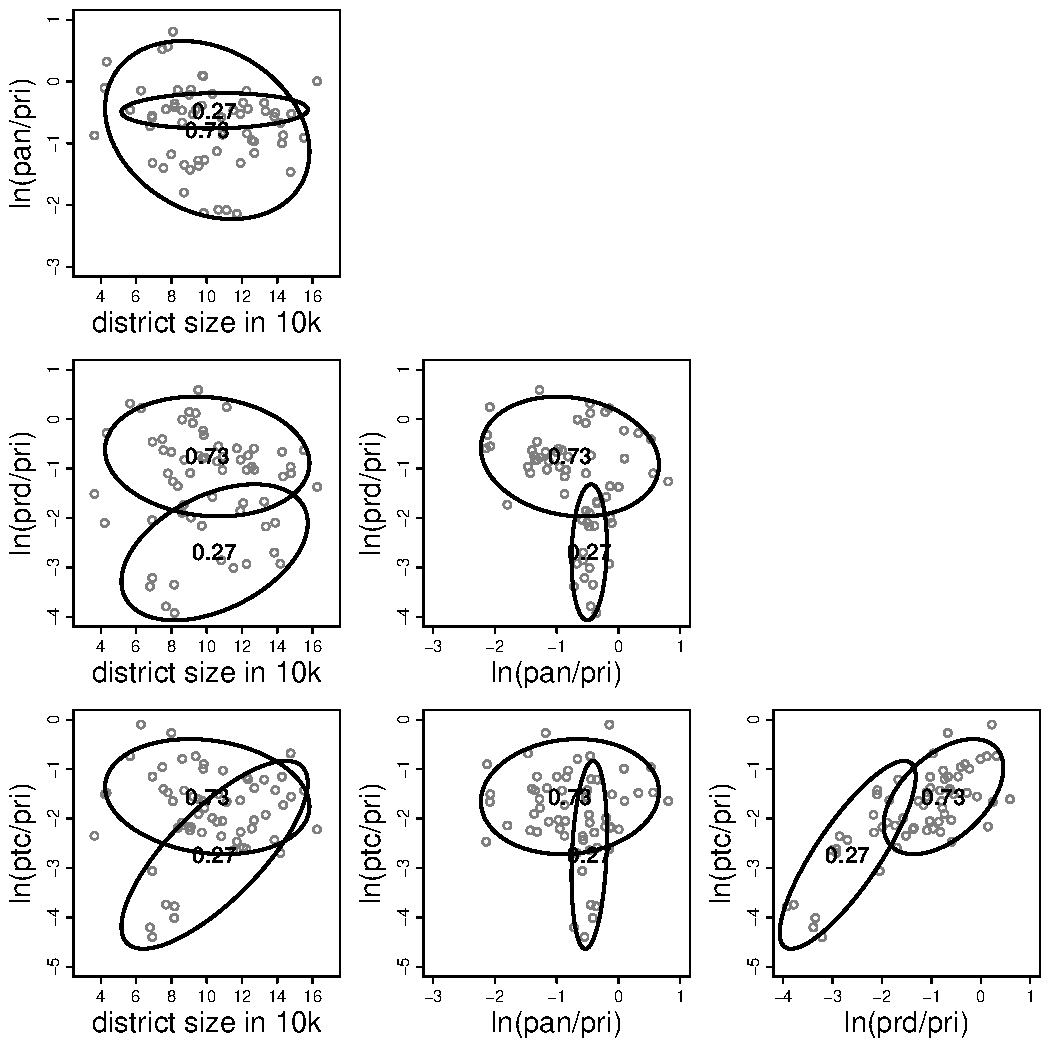
\includegraphics[width=.45\columnwidth]{linzerLogVot2009-1.pdf} &
%     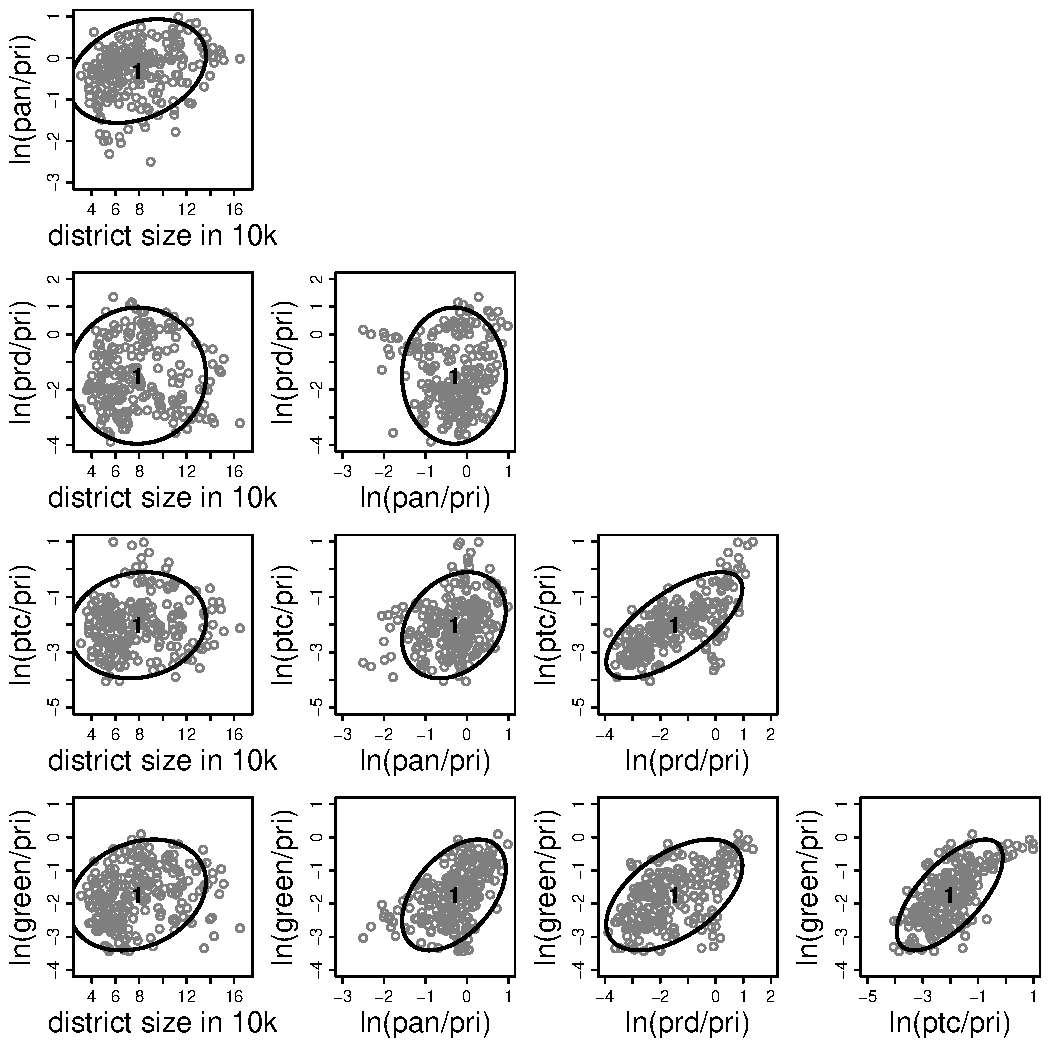
\includegraphics[width=.45\columnwidth]{linzerLogVot2009-2.pdf} 
%   \end{tabular}
%   \caption{Components and mix in the 2009 election. Panels report the log-ratio of party votes, using the PRI as reference to overcome the compositional nature of the data. Circles represent the multi-variate normal distributions that will be combined towards the estimated joint density. Numbers are the relative weights of the components.}\label{F:linzerLogVot}
% \end{center}
% \end{figure}

% \citet{linzerSeatVoteElasticity2012} is a procedure overcoming both complictions with single-election district-level vote returns. The method relies on a finite mixture model for compositional data in order to estimate the joint probability density of parties' level of electoral support across districts. This joint distribution can inform, probabilistically, how changes in a party's vote share translate into losses, or perhaps gains, for the other parties at the district and the national levels, and thus deduce likely seat changes. The procedure extrapolates from the observed district party vote distributions, combining the properties of to or more multivariate normal into a composite density.\footnote{Mention how many components were used for the different contestations patterns in the code.} Figure \ref{F:linzerLogVot} shows (a) use of log-ratio vote shares (relative to PRI) to overcome compositional data bounds; (b) different patterns of pairwise party competition (ln(PRD/PRI) growth without affecting ln(PAN/PRI)). 

% \begin{figure}
% \begin{center}
%     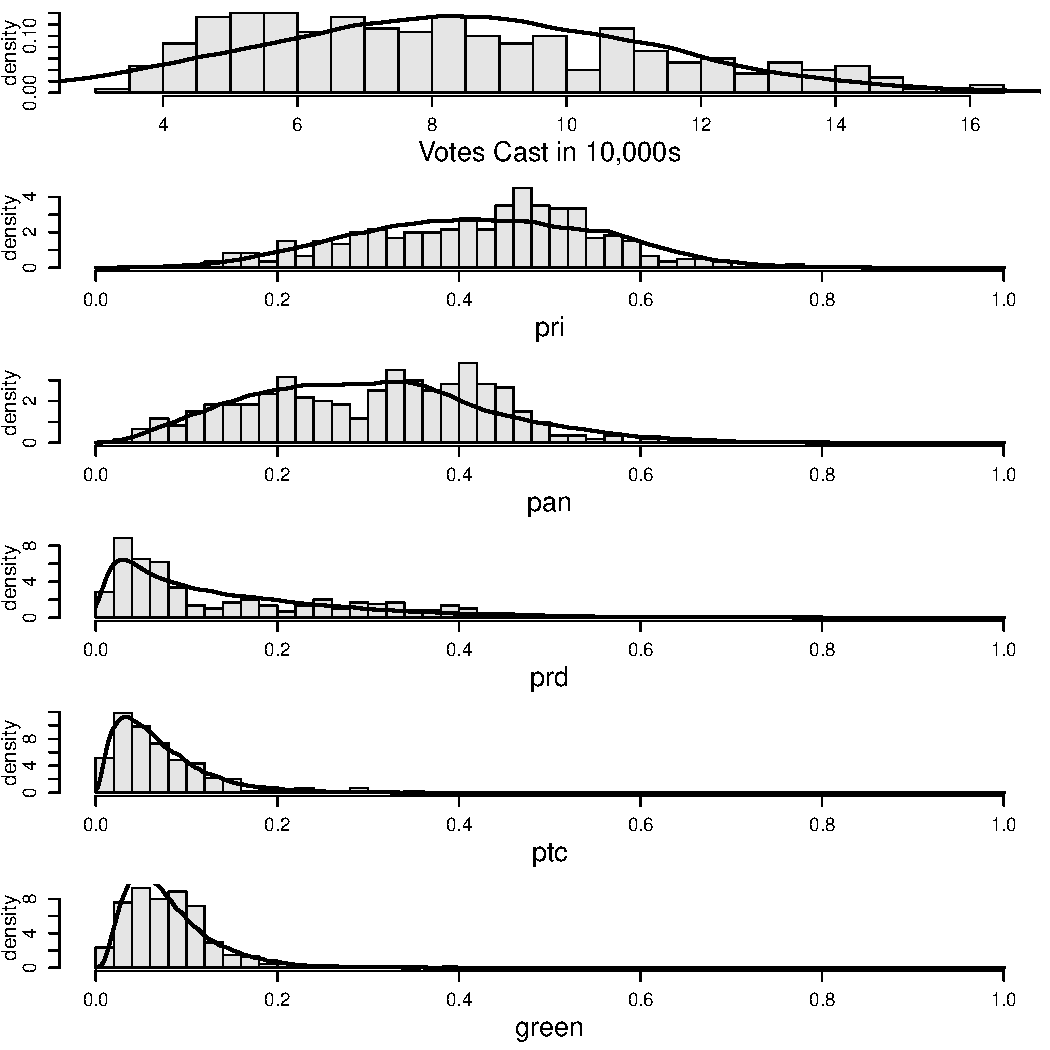
\includegraphics[width=.45\columnwidth]{linzerMarg2009.pdf}
%   \caption{Fit of the finite mixture for 2009. Histograms report actual district party vote shares, lines are the marginals of the estimated 2009 election joint density.}\label{F:linzerMarginals}
% \end{center}
% \end{figure}

% Figure \ref{F:linzerMarginals} to asses fit of estimated joint density. 

% \begin{figure}
% \begin{center}
%   \begin{tabular}{cc}
%     (a) Simulated vote shares & (b) Simulated seat shares \\
%     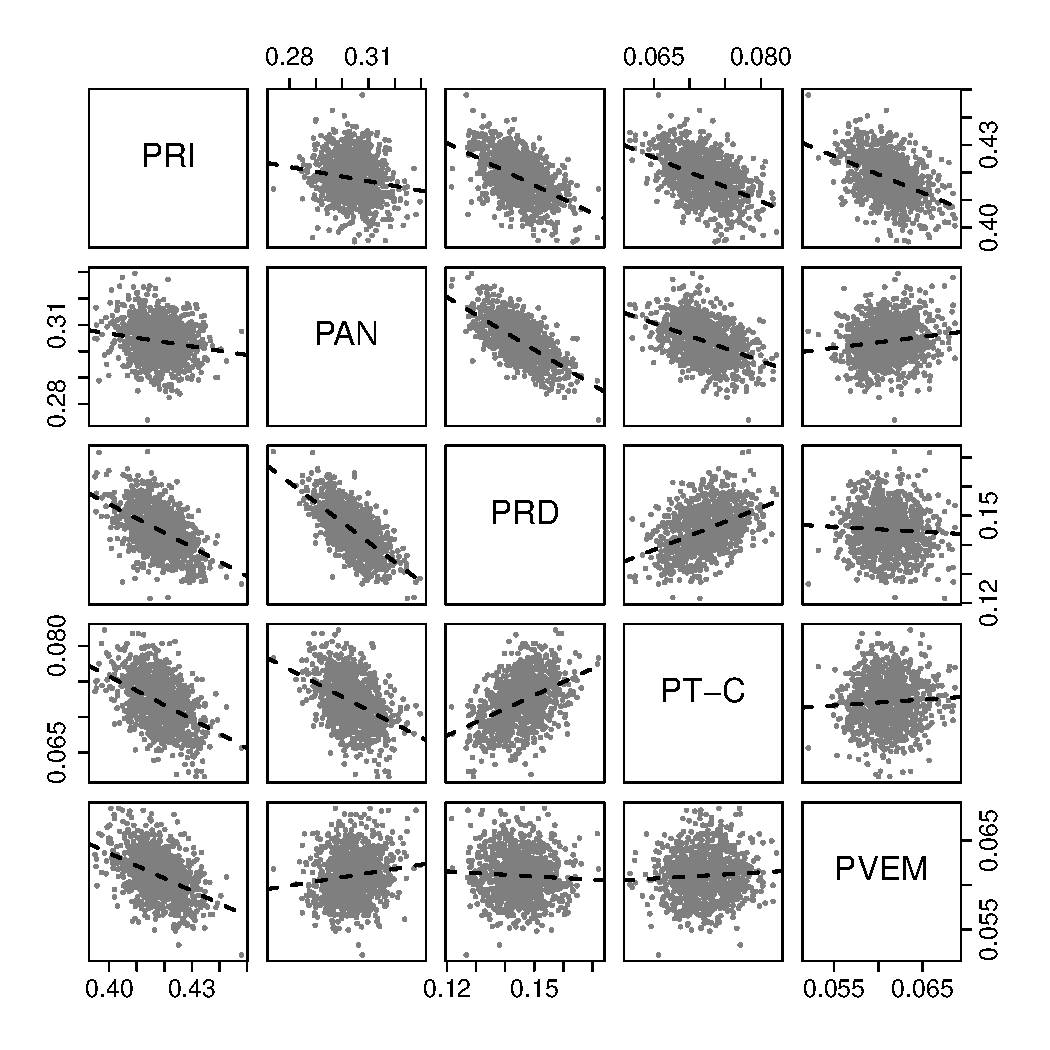
\includegraphics[width=.45\columnwidth]{linzerVoteSims2009.pdf} &
%     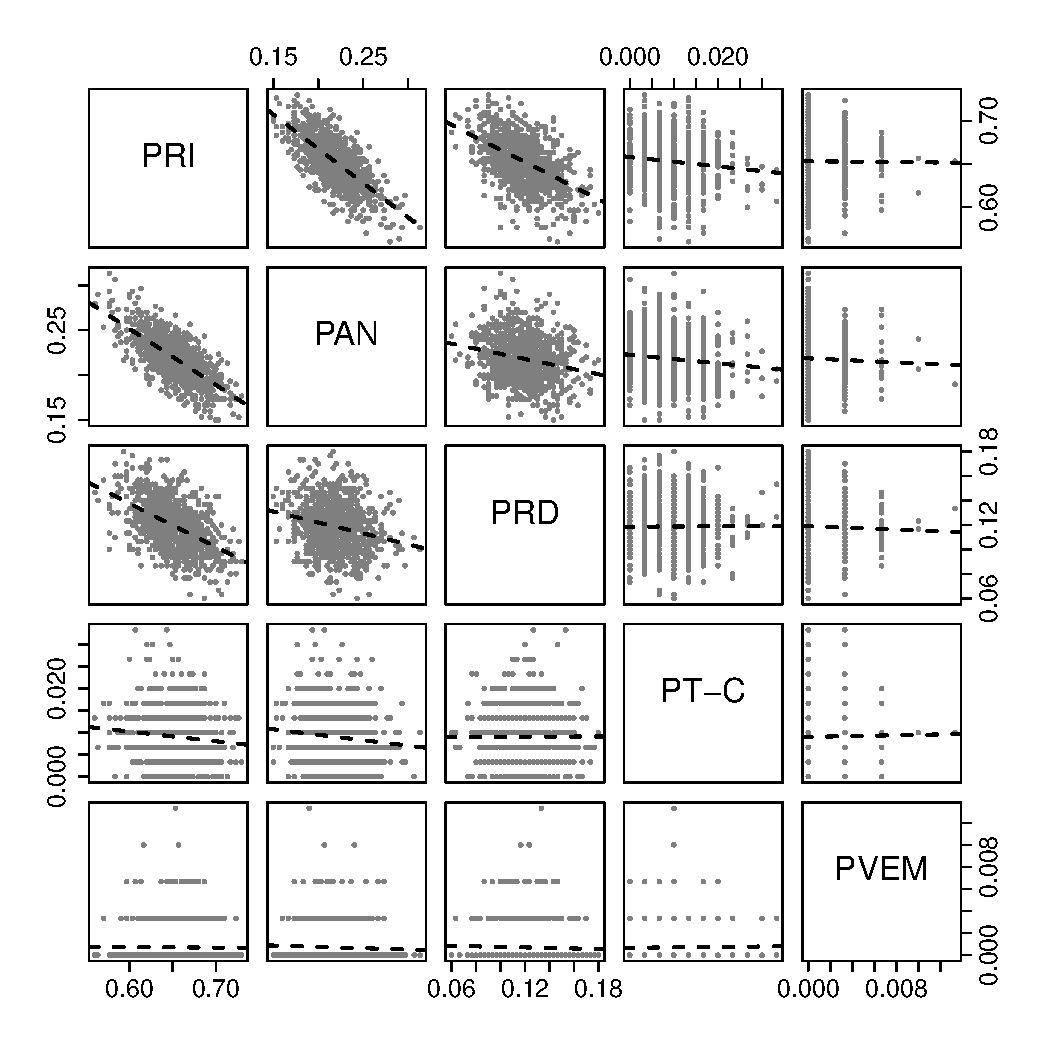
\includegraphics[width=.45\columnwidth]{linzerSeatSims2009.pdf} 
%   \end{tabular}
%   \caption{Covariance of party (a) vote shares and (b) seat shares in the 2009 election. Panels portray 1,000 elections simulated with the Linzer model, and the fit pf a linear regression.}\label{F:linzerSims}
% \end{center}
% \end{figure}

% Monte-Carlo simulation to visit the vote and seat densities, and learn from them. Discuss the 1,000 simulated 2009 elections in Figure {F:linzerSims}. PRD growth votewise correlates with drops in the PRI vote and the PAN vote, but with increases in PT-C votes; PAN and PRD very negative in votes, but not in seats---their marginal districts are not against one another, but against the PRI. 

% Seats--votes simulations for the 2006 and 2015 maps were generated for each election and party separately---single-election analysis offers the advantage of making temporal differences in party swing ratios available. Simulations were pooled, regressing simulates seats on simulated votes, a dummy indicating the 2015 map, and the simulated votes-dummy interaction. This approach has the advangage of offering a test of swing ratio differences attributable to the change in maps. 

% $S_{p,m} = \beta_0 + \beta_1 V_{p,m} + \beta_2 dMap2015_m + \beta_3 V_{p,m} \times dMap2015_m + \texttt{error}_{p,m}$

% \begin{table}
% \centering
% \begin{tabular}{lrrrrrr}
%                    & \mc{2}{c}{PAN}   & \mc{2}{c}{PRI}   & \mc{2}{c}{Left}   \\
%                    & $\hat{\beta}$ & $p$ & $\hat{\beta}$ & $p$ & $\hat{\beta}$ & $p$  \\ \hline
% ~~\textbf{2006 election} \\
% $V$                &     1.94 & $<.001$&   2.27 &$<.001$&   1.91 &$<.001$\\
% $V \times$ dis2015 &     +.45 & $<.001$&  $-.01$&  .809 &  $-.04$&  .183 \\
% ~~\textbf{2009 election} \\
% $V$                &     1.95 & $<.001$&   2.27 &$<.001$&   1.67 &$<.001$\\
% $V \times$ dis2015 &    $-.13$&   .003 &   +.04 &  .354 &  $-.02$&  .623 \\
% ~~\textbf{2012 election} \\
% $V$                &     2.24 &$<.001$ &   3.99 &$<.001$&   2.39 &$<.001$\\
% $V \times$ dis2015 &     +.02 &   .604 &   +.03 &  .720 &  $-.06$&  .103 \\ \hline
% \end{tabular}
% \caption{Comparative 2006 and 2015 map seats--votes swing ratios. $\hat{\beta}$ are estimated coefficients of party seat shares regressed on vote shares ($V$) and vote shares-redistricting interaction ($V \times$ dis2015) and the corresponding $p$-values, using data simulated with the \citet{linzerSeatVoteElasticity2012} finite mixture method. A constant and a redistricting dummy were also included in the right side but are not reported. See text for details.} 
% \end{table}

% \section{Electoral volatility}

% * * To be written * * May help explain why malapportionment has no larger consequences. 

% One factor that may explain the absence of party bias is electoral volatility. By being larger than malapportionment, it may be ecplipsing its potential to create bias...

% Noting a systematic widening of Congressional victory margins in the U.S.\ since the mid-1960s, \citet{mayhew1974vanishingMg} saw gerrymandering as one possible explanation, incumbents influencing the preservation of safe districts. While the argument opened the heated incumbency advantage debate, the intuition may guide our inquiry. District volatility should capture a key element for analysis of map similarities. District $d$ volatility is $v_d = 1/2 \sqrt{ \sum_{p=1}^P \sum_{t=2}^3 (v_{d,p,t}- v_{d,p,t-1})^2 }$ with $p$ indexing the competing parties and $t=1,2,3$ for the 2006,  2009, and 2012 congressional elections respectively.\footnote{The measure of volatility proposed is inspired in measures of disproportionality, replacing the seats--votes difference with vote first differences. It is a squared version of a Loosemore-Hanby index \citep{loosemore.hanbyDisproportionality1971,gallagherDisproportionality1991}.} 

% Mexican party strength is not proportional to the formidable entry barriers they enjoy and massive public subsidies they receive yearly \citep{magar.2007ref.2015}. Evidence of this is their inability to cultivate loyal voters. District volatility is remarkably high, as shown in Table \ref{T:volatMarginsd0}. The median district saw 25 percent of votes change party hands between 2006 and 2012 (not exactly how the index reads, but close enough). With so many volatile districts around, parties should have attempted to redress strongholds that automated redistricting split beyond recognition. How much were strongholds affected by the initial 2015 proposal? To what extent did party counter-proposals redress them? This should be a promising line of inquiry. 

% \begin{table}
% \begin{center}
% \begin{tabular}{lrrrrr}
%                     &  min.   &  25\%   & median  & 75\%   & max \\ \hline
% district volatility &  .08    & .19     & .25     & .31    & .52 \\
% mean PAN margin     &  $-.49$ & $-.23$  & $-.10$  & .01    & .28 \\   
% mean PRI margin     &  $-.43$ & $-.09$  & $-.01$  & .07    & .28 \\   
% mean PRD margin     &  $-.51$ & $-.31$  & $-.21$  & $-.04$ & .39 \\
% \end{tabular}
% \caption{2006 map district volatility and party margins in three congressional elections}\label{T:volatMarginsd0}
% \end{center}
% \end{table}


\section{Conclusion}

% [Micah] We can rewrite this section to focus on the interesting positive findings:
%- malapportionment is substantial
%- there is some persistent overall bias
%- despite a nominally neutral system, the PAN was able to overcome a large turnout disadvantage through more favorable line drawing (gerrymandering)

Inspection of Mexican congressional districts uncovered non-trivial malapportionment---nearly half of district for the midterm congressional in June 2015 will have populations that deviate from the mean district size by more than $\pm30\%$. The problem is built into rules commanding the use of census data to redraw district boundaries, while remaining silent about when drawing must be done. The last three redistricting rounds dragged by more than a half a decade. By then, population data was outdated. 

Fitting a votes--seats curve to measure party bias revealed that the plurality component of Mexico's mixed electoral system gave persistent advantage to some parties in recent congressional elections. Relative to the PAN, there is evidence of small, but systematic bias in favor of the PRI in the votes-to-seats conversion, and of larger, but more volatile bias favorable to the PRD throughout the period. These findings, derived from simulated data to bridge methodological complications, are in contrast with other studies finding no evidence of party bias in state-level data \citep{magar.altman.mcd.trelles2014uh} or evidence of substantive anti-PRI bias in multi-election data \citep{marquez2014biasBlog}. Our findings here are more solidly grounded. **Elaborate how/why.

A breakdown of the components of party bias with \citeauthor{grofman.etalBiasMalapp.1997}'s method adds further depth to our findings. Malapportionment added surprisingly little to the mix. It helped the left relative to other major parties, and with growing strength as maps aged, but the contribution is much smaller than, and easily canceled by those of turnout differences and the geographic distribution of party strength. Despite nominally neutral redistricting, the left in most years, and the PAN in 2006 were able to overcome a large turnout disadvantage through more favorable line drawing. Gerrymandering merits closer inspection in the future. 

%In spite of its meager contribution to party bias, malapportionment remains a fundamental contradiction of the `one person, one vote' principle of democratic government. We therefore encourage reformers to add a simple clause to map makers to redistrict ``as soon as reasonably possible'' (use the language of Supreme Court and British practice). There is no guarantee that future redistricting delays will not begin degrading some parties like they degrade some citizens. 

\section*{Appendix 1: BUGS code}

\singlespacing

\begin{scriptsize}
\begin{verbatim}
bugsModel <- function() {
    for (i in 1:I){     # loop over state-years
        for (p in 1:P){ # loop over parties (dummy selects those who ran that year) 
            S[i,p] ~ dbin(pi[i,p], D[i])  # D is number SMD seats in obs. i's state
        }
        numerator[i,1] <- dummy[i,1] * exp( lambda[1] + rho * log(v[i,1]) )
        numerator[i,2] <- dummy[i,2] * exp(             rho * log(v[i,2]) )
        for (p in 3:P){
            numerator[i,p] <- dummy[i,p] * exp( lambda[p-1] ) * v[i,p]^rho
        }
        for (p in 1:P){ # loop over parties (dummy=1 selects those who ran that year) 
            d1[i,p] <- dummy[i,1] * exp( lambda[1] ) * v[i,1]^rho 
            d2[i,p] <- dummy[i,2]                    * v[i,2]^rho 
            d3[i,p] <- dummy[i,3] * exp( lambda[2] ) * v[i,3]^rho 
            d4[i,p] <- dummy[i,4] * exp( lambda[3] ) * v[i,4]^rho 
            d5[i,p] <- dummy[i,5] * exp( lambda[4] ) * v[i,5]^rho 
            d6[i,p] <- dummy[i,6] * exp( lambda[5] ) * v[i,6]^rho 
            d7[i,p] <- dummy[i,7] * exp( lambda[6] ) * v[i,7]^rho 
            denominator[i,p] <- d1[i,p]+d2[i,p]+d3[i,p]+d4[i,p]+d5[i,p]+d6[i,p]+d7[i,p]
            pi[i,p] <- numerator[i,p] / denominator[i,p]
        }
    }
    ### priors
    for (q in 1:6){ # there are 7 party labels in the 3-election data, PRI is reference
        lambda[q] ~ dnorm( 0, tau.lambda )
    }
    tau.lambda <- pow(.25, -2)
    rho ~ dexp(.75) # this has positive range, median close to 1, mean 1.25, max 4.5
}
\end{verbatim}
\end{scriptsize}

\onehalfspacing


\bibliographystyle{apsr}
%\bibliography{../bib/redMex}
\bibliography{../bib/magar}

%% next command, in console, extracts only relevant paper references to extracted.bib (http://tex.stackexchange.com/questions/41821)
%bibexport -o extracted.bib myarticle.aux

\end{document}
